
\documentclass[10pt,twocolumn,letterpaper]{article}

%%%%%%%%% PAPER TYPE  - PLEASE UPDATE FOR FINAL VERSION
% \usepackage[review]{cvpr}      % To produce the REVIEW version
% \usepackage{cvpr}              % To produce the CAMERA-READY version
\usepackage[pagenumbers]{cvpr} % To force page numbers, e.g. for an arXiv version

% Include other packages here, before hyperref.
\usepackage{graphicx}
\usepackage{amsmath}
\usepackage{amssymb}
\usepackage{booktabs}
\usepackage{mathalias}
\usepackage{multirow}
\usepackage{bbm}
\usepackage{caption}
\usepackage[table]{xcolor}
\usepackage{color}
\usepackage{pifont}
\usepackage{pifont}
\usepackage{algorithm}
\usepackage{listings}
\usepackage{placeins}
\usepackage[accsupp]{axessibility} 

\newcommand{\name}{CaSSLe}
\newcommand\inlineeqno{\stepcounter{equation}\ (\theequation)}


\renewcommand{\baselinestretch}{0.98}

\newcommand{\CC}[1]{\cellcolor{#1}}
\definecolor{ftcolor}{rgb}{1,1,1} % almond
\definecolor{baselinecolor}{rgb}{1,1,1}
\definecolor{contrcolor}{rgb}{1.0, 0.98, 0.8}
\definecolor{predcolor}{rgb}{0.74, 0.83, 0.9}
\definecolor{decorrcolor}{rgb}{0.98, 0.85, 0.87} % palepink
\definecolor{knowcolor}{rgb}{0.82, 0.94, 0.75}
\definecolor{offlinecolor}{rgb}{1,1,1}
\definecolor{firsttaskcolor}{rgb}{0.97, 0.97, 0.97}
\definecolor{azure(colorwheel)}{rgb}{0.0, 0.5, 1.0}

\newcommand*\samethanks[1][\value{footnote}]{\footnotemark[#1]}

\usepackage[pagebackref,breaklinks,colorlinks=true,allcolors=blue]{hyperref}


% Support for easy cross-referencing
\usepackage[capitalize]{cleveref}
\crefname{section}{Sec.}{Secs.}
\Crefname{section}{Section}{Sections}
\Crefname{table}{Table}{Tables}
\crefname{table}{Tab.}{Tabs.}


%%%%%%%%% PAPER ID  - PLEASE UPDATE
\def\cvprPaperID{****} % *** Enter the CVPR Paper ID here
\def\confName{****}
\def\confYear{****}

\newcommand{\mybullet}{\raisebox{1.5pt}{\scriptsize $\blacktriangleright$}}

\begin{document}

%%%%%%%%% TITLE - PLEASE UPDATE
\title{Self-Supervised Models are Continual Learners}

\author{Enrico Fini\thanks{\scriptsize{Enrico Fini and Victor G. Turrisi da Costa contributed equally.}} \,$^{\textcolor{azure(colorwheel)}{1,2}}$ \quad Victor G. Turrisi da Costa\samethanks \, $^{\textcolor{azure(colorwheel)}{1}}$ \quad Xavier Alameda-Pineda$^{\textcolor{azure(colorwheel)}{2}}$\\
Elisa Ricci$^{\textcolor{azure(colorwheel)}{1,3}}$ \quad Karteek Alahari$^{\textcolor{azure(colorwheel)}{2}}$ \quad Julien Mairal$^{\textcolor{azure(colorwheel)}{2}}$\vspace{5px}\\
\normalsize{$^{\textcolor{azure(colorwheel)}{1}}$ University of Trento \quad $^{\textcolor{azure(colorwheel)}{2}}$ Inria\thanks{\scriptsize{Univ. Grenoble Alpes, CNRS, Grenoble INP, LJK, 38000 Grenoble, France.}} \quad $^{\textcolor{azure(colorwheel)}{3}}$ Fondazione Bruno Kessler}
}
\maketitle

%%%%%%%%% ABSTRACT
\begin{abstract}
Self-supervised models have been shown to produce comparable or better visual representations than their supervised counterparts when trained offline on unlabeled data at scale. However, their efficacy is catastrophically reduced in a Continual Learning (CL) scenario where data is presented to the model sequentially. In this paper, we show that self-supervised loss functions can be seamlessly converted into distillation mechanisms for CL by adding a predictor network that maps the current state of the representations to their past state. This enables us to devise a framework for Continual self-supervised visual representation Learning that (i) significantly improves the quality of the learned representations, (ii) is compatible with several state-of-the-art self-supervised objectives, and (iii) needs little to no hyperparameter tuning. We demonstrate the effectiveness of our approach empirically by training six popular self-supervised models in various CL settings. Code: \href{https://github.com/DonkeyShot21/cassle}{\texttt{github.com/DonkeyShot21/cassle}}.
\end{abstract}\

%%%%%%%%% BODY TEXT
\section{Introduction}
\label{sec:intro}


Transformers, in particular decoder-only models (e.g.\ GPT~\citep{brown2020language}, Llama~\citep{touvron2023llama}) which process input sequences in a causal fashion, are one of the main drivers of modern deep learning's success.
Numerous approaches attempt to approximate the core attention layer to address its efficiency issues~\citep{tay2022efficient}, such as scaling quadratically in sequence length during training and requiring a cache of size linear in sequence length during autoregressive generation.
In parallel, a class of alternative sequence models, structured state-space models (SSMs), have emerged with linear scaling in sequence length during training and constant state size during generation.
They show strong performance on long-range tasks (e.g. S4~\citep{gu2022efficiently}) and recently matched or beat Transformers on language modeling (e.g. Mamba \citep{gu2023mamba}) at small to moderate scale.
However, the development of SSMs have appeared disjoint from the community's collective effort to improve Transformers, such as understanding them theoretically as well as optimizing them on modern hardware.
As a result, it is more difficult to understand and experiment with SSMs compared to Transformers, and it remains challenging to train SSMs as efficiently as Transformers from both an algorithmic and systems perspective.


Our main goal is to develop a rich body of theoretical connections between structured SSMs and variants of attention.
This will allow us to transfer algorithmic and systems optimizations originally developed for Transformers to SSMs, towards the goal of building foundation models that perform better than Transformers while scaling more efficiently in sequence length.
A milestone contribution in this direction was the \textbf{Linear Attention (LA)} framework \citep{katharopoulos2020transformers},
which derived a connection between autoregressive attention and linear RNNs
by showing the equivalence between ``dual forms'' of quadratic kernelized attention and a particular linear recurrence.
This duality allows new capabilities such as the ability to have both efficient parallelizable training and efficient autoregressive inference.
In the same spirit, this paper provides multiple viewpoints connecting linear-complexity SSMs with quadratic-complexity forms to combine the strengths of SSMs and attention.%
\footnote{Technically speaking, these connections only relate to certain flavors of attention; the title of this paper is an homage to \citet{katharopoulos2020transformers} which first showed that ``Transformers are RNNs''.}

\iftoggle{arxiv}{
\begin{wrapfigure}{R}{0.48\linewidth}
  \begin{center}
    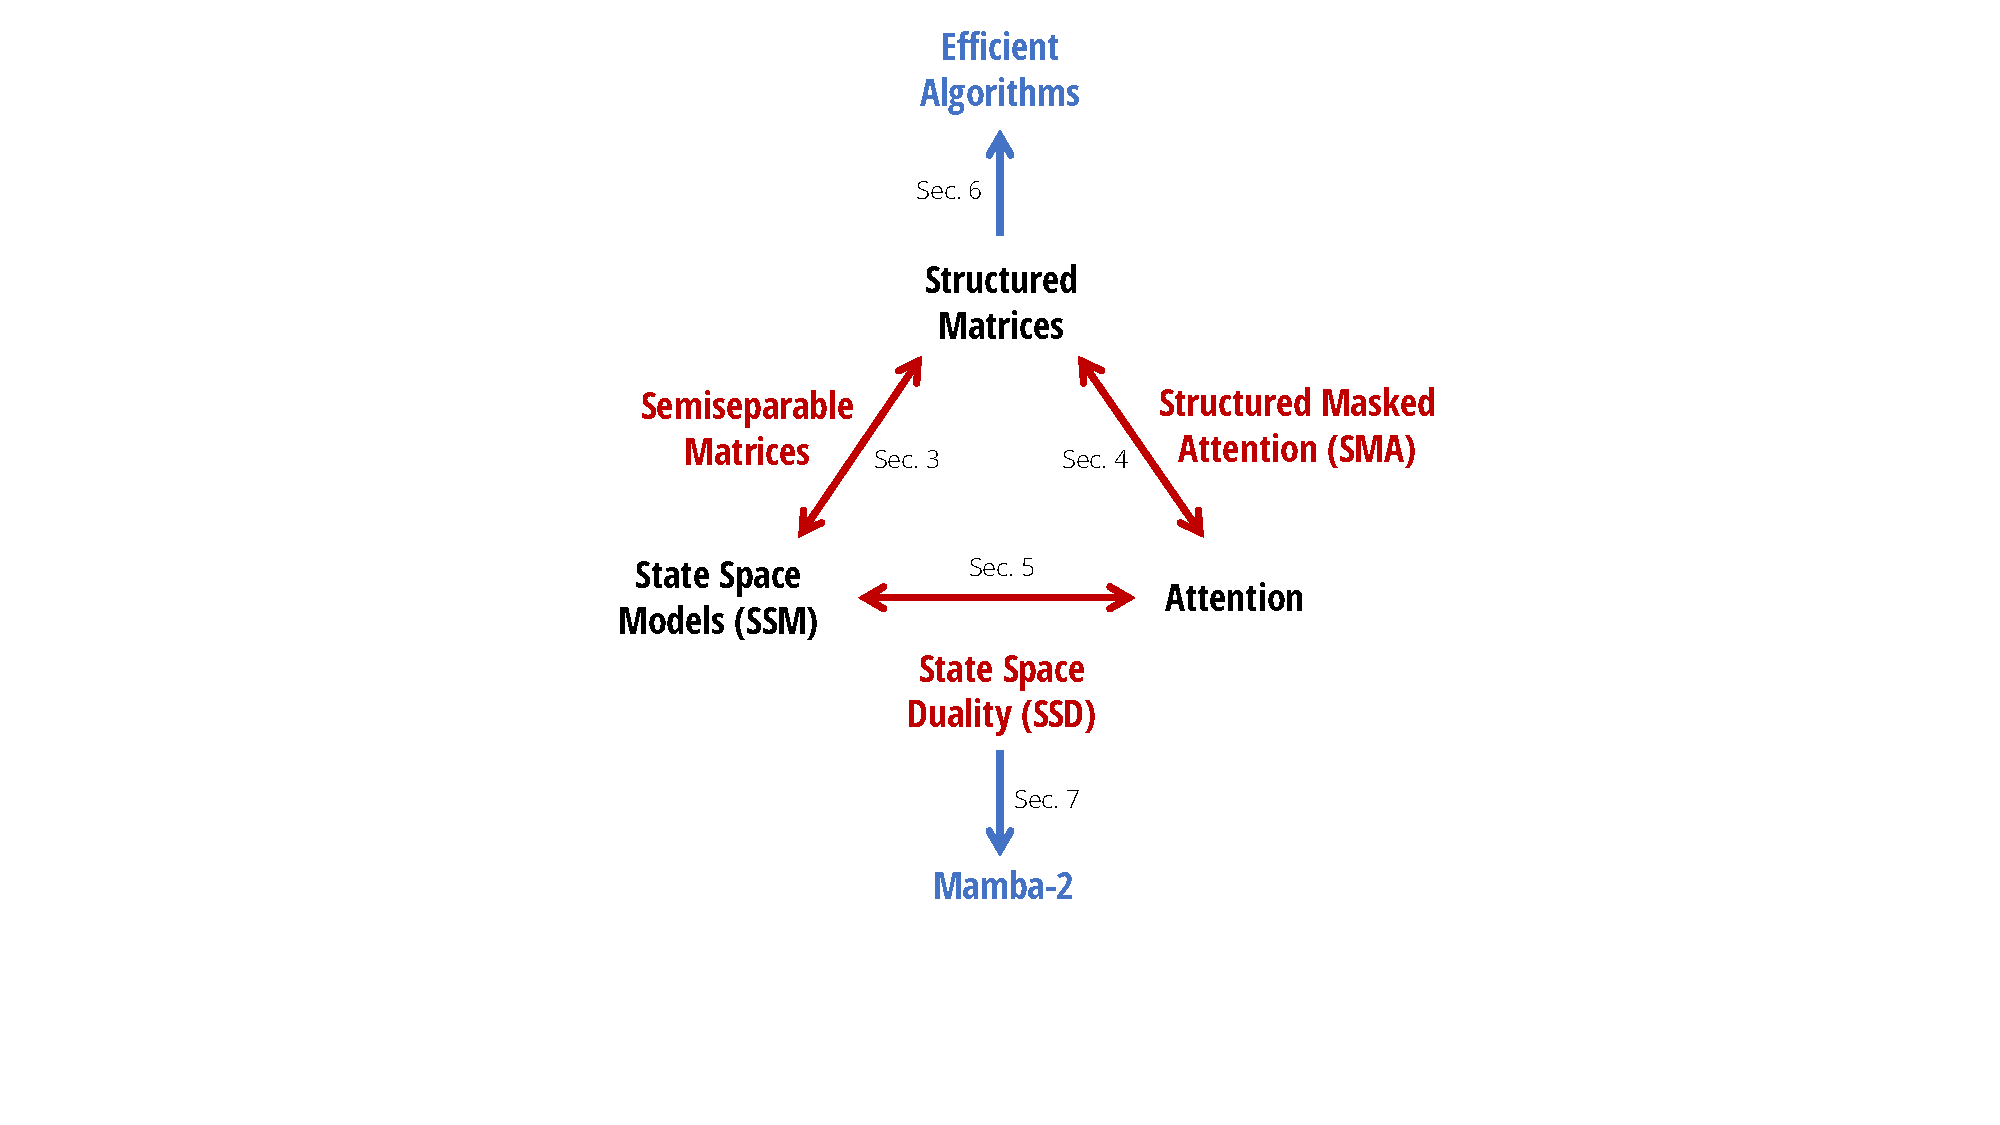
\includegraphics[width=\linewidth]{fig/ssd_roadmap.pdf}
  \end{center}
  \caption{
    (\textbf{Structured State-Space Duality}.)
    This paper fleshes out the relationship between state space models and attention through the bridge of structured matrices.
  }
  \label{fig:roadmap}
\end{wrapfigure}
}{}

\para{State Space Duality.}
Our framework connecting structured SSMs and variants of attention, which we call \textbf{structured state space duality} (SSD),
is made through the abstractions of \textbf{structured matrices}:
matrices with subquadratic parameters and multiplication complexity.
We develop two broad frameworks for representing sequence models, one as matrix transformations and one as tensor contractions, which each reveal different perspectives of the duality.
Our technical contributions include:
\begin{itemize}[leftmargin=*,itemsep=0pt,topsep=0pt]
  \item We show an equivalence between state space models and a well-studied family of structured matrices called \textbf{semiseparable matrices}\iftoggle{arxiv}{ (\cref{sec:ssm})}{}.
    This connection is at the heart our framework, revealing new properties and algorithms for SSMs. A central message of this paper is that \emph{different methods of computing state space models can be reframed as various matrix multiplication algorithms on structured matrices}.
  \item We significantly improve the theory of linear attention~\citep{katharopoulos2020transformers}.
    We first provide an incisive proof of its recurrent form through the language of tensor contractions, and then generalize it to a new family of \textbf{structured masked attention (SMA)}\iftoggle{arxiv}{ (\cref{sec:attention})}{}.
  \item We connect SSMs and SMA, showing that they have a large intersection that are duals of each other, possessing both SSM-like linear and attention-like quadratic forms\iftoggle{arxiv}{ (\cref{sec:ssd})}{}.
    \iftoggle{arxiv}{We also prove that any kernel attention method possessing a fast recurrent form must be an SSM.}{}
\end{itemize}


Beyond its intrinsic theoretical value, our framework opens up a broad set of directions for understanding and improving sequence models.

\para{Efficient Algorithms.}
First and most importantly, our framework exposes new efficient and easily-implementable algorithms for computing SSMs\iftoggle{arxiv}{ (\cref{sec:efficient})}{}.
We introduce a new \textbf{SSD algorithm}, based on block decompositions of semiseparable matrices, that takes advantage of both the linear SSM recurrence and quadratic dual form, obtaining optimal tradeoffs on all main efficiency axes (e.g. training and inference compute, memory usage, and ability to leverage matrix multiplication units on modern hardware).
A dedicated implementation of SSD is $2-8\times$ faster than the optimized selective scan implementation of Mamba, while simultaneously allowing for much larger recurrent state sizes ($8\times$ the size of Mamba or even higher, with minimal slowdown).
SSD is highly competitive with optimized implementations of softmax attention (FlashAttention-2~\citep{dao2023flashattention2}), crossing over at sequence length 2K and 6$\times$ faster at sequence length 16K.


\iftoggle{arxiv}{
\para{Architecture Design.}
One major obstacle to adopting new architectures such as SSMs is the ecosystem tailored to Transformers, such as hardware-efficient optimization and parallelism techniques for large-scale training.
Our framework allows using established conventions and techniques for attention to build a vocabulary of architecture design choices for SSMs, and further improve them (\cref{sec:architecture}).
For example, we introduce the analog of heads from multi-head attention (MHA) to SSMs.
We show that the Mamba architecture is a \textbf{multi-input SSM (MIS)} that turns out to be analogous to \textbf{multi-value attention (MVA)}, and compare other variants of Mamba with different head structures.

We also use these ideas to make slight modifications to the Mamba block, which allows tensor parallelism to be implemented (e.g. in the style of Megatron~\citep{shoeybi2019megatron}).
The main ideas include introducing grouped-value attention (GVA) head structure, and moving all data-dependent projections to occur in parallel at the beginning of the block.


}{
  \para{Mamba-2.}
  Additionally, inspired by the connection between SSMs and Transformers, we slightly modify the neural network architecture of Mamba by moving all data-dependent projections to occur in parallel at the beginning of the block. %
}
The combination of the modified parallel Mamba block, together with using SSD as the inner SSM layer, results in the \textbf{Mamba-2} architecture.
We investigate Chinchilla scaling laws for Mamba-2 in the same setting as Mamba, finding that it Pareto dominates Mamba and Transformer++ in both perplexity and wall-clock time.
We additionally train a family of Mamba-2 models at varying sizes on the Pile, showing that it matches or outperforms Mamba and open source Transformers on standard downstream evaluations.
For example, Mamba-2 with 2.7B parameters trained on 300B tokens on the Pile outperforms Mamba-2.8B, Pythia-2.8B and even Pythia-6.9B trained on the same dataset.

\iftoggle{arxiv}{
\paragraph{Systems Optimizations.}
The SSD framework connects SSMs and Transformers, allowing us to leverage a rich body of work on systems optimizations developed for Transformers~(\cref{sec:systems}).
\begin{itemize}[leftmargin=*,itemsep=0pt,topsep=0pt]
  \item For example, Tensor Parallelism (TP) is an important model parallelism technique to train large Transformer models by splitting each layer across GPUs on the same node.
    We design Mamba-2 to be TP-friendly, reducing the number of synchronization point per block by half.
  \item For very long sequences whose activations do not fit on one device, sequence parallelism has been developed for the attention blocks.
    We describe how to train SSMs in general and Mamba-2 in particular with sequence parallelism, by passing the recurrent states between devices.
  \item For finetuning with examples of different lengths, for best efficiency, Transformer requires sophisticated techniques to remove padding tokens and perform attention on variable length sequences.
    We show how Mamba-2 can be trained with variable sequence lengths efficiently, requiring no padding tokens.
\end{itemize}
}{}

\cref{sec:experiments} empirically validates Mamba-2 on language modeling, training efficiency, and a difficult multi-query associative recall task~\citep{arora2024simple}.
Finally, in \cref{sec:related}, we provide an extended related work and discuss potential research directions opened up by our framework.

Model code and pre-trained checkpoints are open-sourced at \url{https://github.com/state-spaces/mamba}.






\section{Related work}

There is a rich prior literature on 
probabilistic programming languages (PPLs),
which extend probabilistic graphical models to
support more complex joint distributions whose size and ``shape''
can itself be stochastic (e.g., a graph
unrolled for a random number of iterations,
until a data-dependent stopping criterion is met).
PPLs extend traditional programming languages with the ability to {\it sample} from distributions and {\it observe} values of variables based on data (i.e. condition the model).
The semantics of sample and observe vary depending on the inference algorithm.
For more details, see  \citet{intro_ppl}.

Recently there has been an explosion of interest in large language models, such as 
GPT-3 \citep{gpt3} and PaLM \citep{palm}.
%\citep{lamda}.
These can be used for tasks such as ``zero-shot"
question-answering. In this setting, we 
provide the question $Q$ as a prompt to the LM,
and then sample answers from the model, 
which we denote by $p(A|Q,\theta)$,
where $\theta$ are the pre-trained model parameters.
Alternatively, we can compute the MAP answer,
$\hat{A} = \argmax_A p(A|Q,\theta)$.


To ensure the model ``does the right thing'',
we can provide a small training set of question-answer pairs,
$D = \{ (Q^m,A^m): m=1:M\}$ pairs.
This can be provided as extra context to the model,
provided in the text prompt, followed by sampling
from $p(A|Q,D,\theta)$.
We refer to this as ``few-shot prompting''.
We can also fine-tune the model parameters on $D$ to
get $\theta'$, and then sample
from $p(A|Q,\theta')$.

%We can improve performance on question answering tasks by encouraging the model
%chaining multiple LMs together,  % david: They don't actually do multiple calls, just prompt it to produce the aux variable directly.
%as illustrated in the
%Scratchpad \citep{scratchpads} and Chain of Thought \citep{chainofthought}  papers.
%These papers introduce an  an additional auxiliary ``thought''
%variable $T$ and then extend the model to have the form
%$P(A,T|Q) = P(A|T,Q)P(T|Q)$, where each conditional is computed
%using an LM.

We can improve performance by introducing an additional auxiliary ``thought'' variable,
and then extend the model to have the form $p(A,T|Q) = p(A|T,Q)p(T|Q)$, where each conditional is computed using an LM which includes its conditioning variables as a part of its input.
Work on scratchpads \citep{scratchpads} and chain of thought \citep{chainofthought} illustrate this, and finetune or prompt the LM to produce this auxiliary thought before answering.
%We can improve performance on question answering tasks by encouraging the model
%chaining multiple LMs together,  % david: They don't actually do multiple calls, just prompt it to produce the aux variable directly.
% These papers 
% variable $T$ 

We typically condition this on a small set
$D_S$ of  $(A^m,T^m,Q^m)$ triples,
and optionally a larger set $D_L$ of $(A^m, Q^m)$ pairs.
We then compute a distribution over answers to a test question
using
\begin{align}
\hat{p}(A|Q) = \sum_T 
\hat{p}(A|Q, T) \hat{p}(T|Q)
\label{eqn:probQA}
\end{align}
where $\hat{p}(\cdot) = p(\cdot|D_L,D_S,\theta)$
is the prior predictive distribution. (Scratchpad creates its prior predictive by fine-tuning, while Chain of Thought adds $D_S$ to the LM prompt.)

In practice, we cannot sum over all possible strings $T$
in \cref{eqn:probQA}.
The most common approach is to compute the MAP estimate
$\hat{T} = \argmax \hat{p}(T)$ using beam search,
and then to approximate the sum over $T$ with this single
value.
More recently, Self Consistency \citep{selfconsistency} 
proposed to sample multiple values for $T$
using forward sampling of $(A,T)$ given $Q$,
and then taking the answer $A$ that is most common
in this set\footnote{This bucketing is practical because most standard benchmarks have answers that are just a couple words.}.

PromptChainer \citep{promptchainer} proposes a visual interface for composing language models together, specifying control flow and prompting strategies for each node in a chain. Nodes may query language models or external systems. 
Socratic models \citep{socraticmodels} extends model chaining to the multimodal setting and demonstrates zero-shot abilities on tasks for which no single model exists.

The Eliciting Latent Knowledge proposal \citep{ELK} suggests making latent variables explicit, modelled using a Bayesian network, to improve interpretability and safety for advanced AI systems.
% Factored cognition \citet{factored_cognition}

\citet{ortega2021shaking} explains a formalism for LM finetuning with causal graphical models in order to extend the predictive capabilities of AI agents towards more adaptive behaviour. They focus on analysing an auto-regressive action (random variable) prediction scheme in the interactive setting of RL where a model is simultaneously a generator and predictor of data.

% \citet{language_feedback} incorporates language feedback to finetune models, and finds that learning is significantly more sample efficient. \ddohan{We view this feedback as an auxiliary variable which can be conditioned to inform inference.}

%\kevin{Omit RL refs since not relevant?}
%Incorporating human feedback into generative models remains an open problem. Reinforcement from human feedback has become a popular approach to finetuning models against human preferences. \citep{learning_to_summarize, anthropic_human_feedback} learn a surrogate model of human preferences and use PPO \citep{ppo} to finetune a language model to maximize this surrogate. Rather than using scalar feedback, \citet{language_feedback} incorporates language feedback to finetune models, and finds that learning is significantly more sample efficient. \ddohan{We view this feedback as an auxiliary variable which can be conditioned to inform inference.}
%\todo{ddohan: consider adding back in language feedback ref}

%\citep{Levine2022} presents some very recent work on using frozen LMs in various ways.\rif{Suggest we cut this if we don't have more to say.}






\section{Methodology}
\ours follows the same framework as speculative decoding, where each decoding step primarily consists of three substeps: (1) generating candidates, (2) processing candidates, and (3) accepting candidates. For \ours, (1) is achieved by \ours heads, (2) is realized by tree attention, and since \ours heads are on top of the original model, the logits calculated in (2) can be used for substep (1) for the next decoding step. The final step (3) can be realized by either rejection sampling~\citep{leviathan2022fast,chen2023accelerating} or typical acceptance (Section~\ref{sec:typical_acceptance}). The overall pipeline is illustrated in Figure~\ref{fig:pipeline}.

In this section, we first introduce the key components of \ours, including \ours heads, and tree attention. Then, we present two levels of fine-tuning procedures for \ours to meet the needs of different use cases. Finally, we propose two extensions to \ours, including self-distillation and typical acceptance, to handle situations where no training data is available for \ours and to improve the efficiency of the decoding process, respectively.
\subsection{Key Components}
\subsubsection{\ours Heads}
\label{sec:medusa_heads}
In speculative decoding, subsequent tokens are predicted by an auxiliary draft model. This draft model must be small yet effective enough to generate continuations that the original model will accept. Fulfilling these requirements is a challenging task, and existing approaches~\citep{spector2023accelerating,miao2023specinfer} often resort to separately \emph{pre-training} a smaller model. This pre-training process demands substantial additional computational resources. For example, in \citep{miao2023specinfer}, a reported 275 NVIDIA A100 GPU hours were used. Additionally, separate pre-training can potentially create a distribution shift between the draft model and the original model, leading to continuations that the original model may not favor. \citet{chen2023accelerating} have also highlighted the complexities of serving multiple models in a distributed environment.

\textcolor{black}{To streamline and democratize the acceleration of LLM inference, we take inspiration from \citet{stern2018blockwise}, which utilizes parallel decoding for tasks such as machine translation and image super-resolution. \ours heads}
 are additional decoding heads appended to the last hidden states of the original model. Specifically, given the original model's last hidden states $h_t$ at position $t$, we add $K$ decoding heads to $h_t$. The $k$-th head is used to predict the token in the $(t+k+1)$-th position of the next tokens (the original language model head is used to predict the $(t+1)$-th position). The prediction of the $k$-th head is denoted as $p_t^{(k)}$, representing a distribution over the vocabulary, while the prediction of the original model is denoted as $p_t^{(0)}$. Following the approach of \citet{stern2018blockwise}, we utilize a single layer of feed-forward network with a residual connection for each head. We find that this simple design is sufficient to achieve satisfactory performance. The definition of the $k$-th head is outlined as:

\begin{align*}
p_t^{(k)} = \text{softmax}\left(W_2^{(k)} \cdot \left(\text{SiLU}(W_1^{(k)} \cdot h_t)+h_t\right)\right),\\
\text{where } W_2^{(k)}\in\mathbb{R}^{d\times V}, W_1^{(k)}\in\mathbb{R}^{d\times d}.
\end{align*}

\textcolor{black}{$d$ is the output dimension of the LLM's last hidden layer and $V$ is the vocabulary size.}
\textcolor{black}{We initialize $W_2^{(k)}$ identically to the original language model head, and $W_1^{(k)}$ to zero.}
This aligns the initial prediction of \ours heads with that of the original model. The SiLU activation function~\citep{elfwing2017sigmoidweighted} is employed following the Llama models~\citep{touvron2023llama}.

Unlike a draft model, \ours heads are trained in conjunction with the original backbone model, which can remain \emph{frozen} during training (\ours-1) or be trained together (\ours-2). This method allows for fine-tuning large models even on a single GPU, taking advantage of the powerful base model's learned representations. Furthermore, it ensures that the distribution of the \ours heads aligns with that of the original model, thereby mitigating the distribution shift problem. Additionally, since the new heads consist of just a single layer akin to the original language model head, \ours does not add complexity to the serving system design and is friendly to distributed settings. We will discuss the training recipe for \ours heads in Section~\ref{sec:training_recipe}.

\subsubsection{Tree Attention}
\label{sec:tree_attention}
Through \ours heads, we obtain probability predictions for the subsequent $K+1$ tokens. These predictions enable us to create length-$K+1$ continuations as candidates. While the speculative decoding studies~\citep{leviathan2022fast,chen2023accelerating} suggest sampling a single continuation as the candidate, leveraging multiple candidates during decoding can enhance the expected acceptance length within a decoding step. Nevertheless, more candidates can also raise computational demands. To strike a balance, we employ a tree-structured attention mechanism to process multiple candidates concurrently.
\begin{figure}[ht]
    \centering
    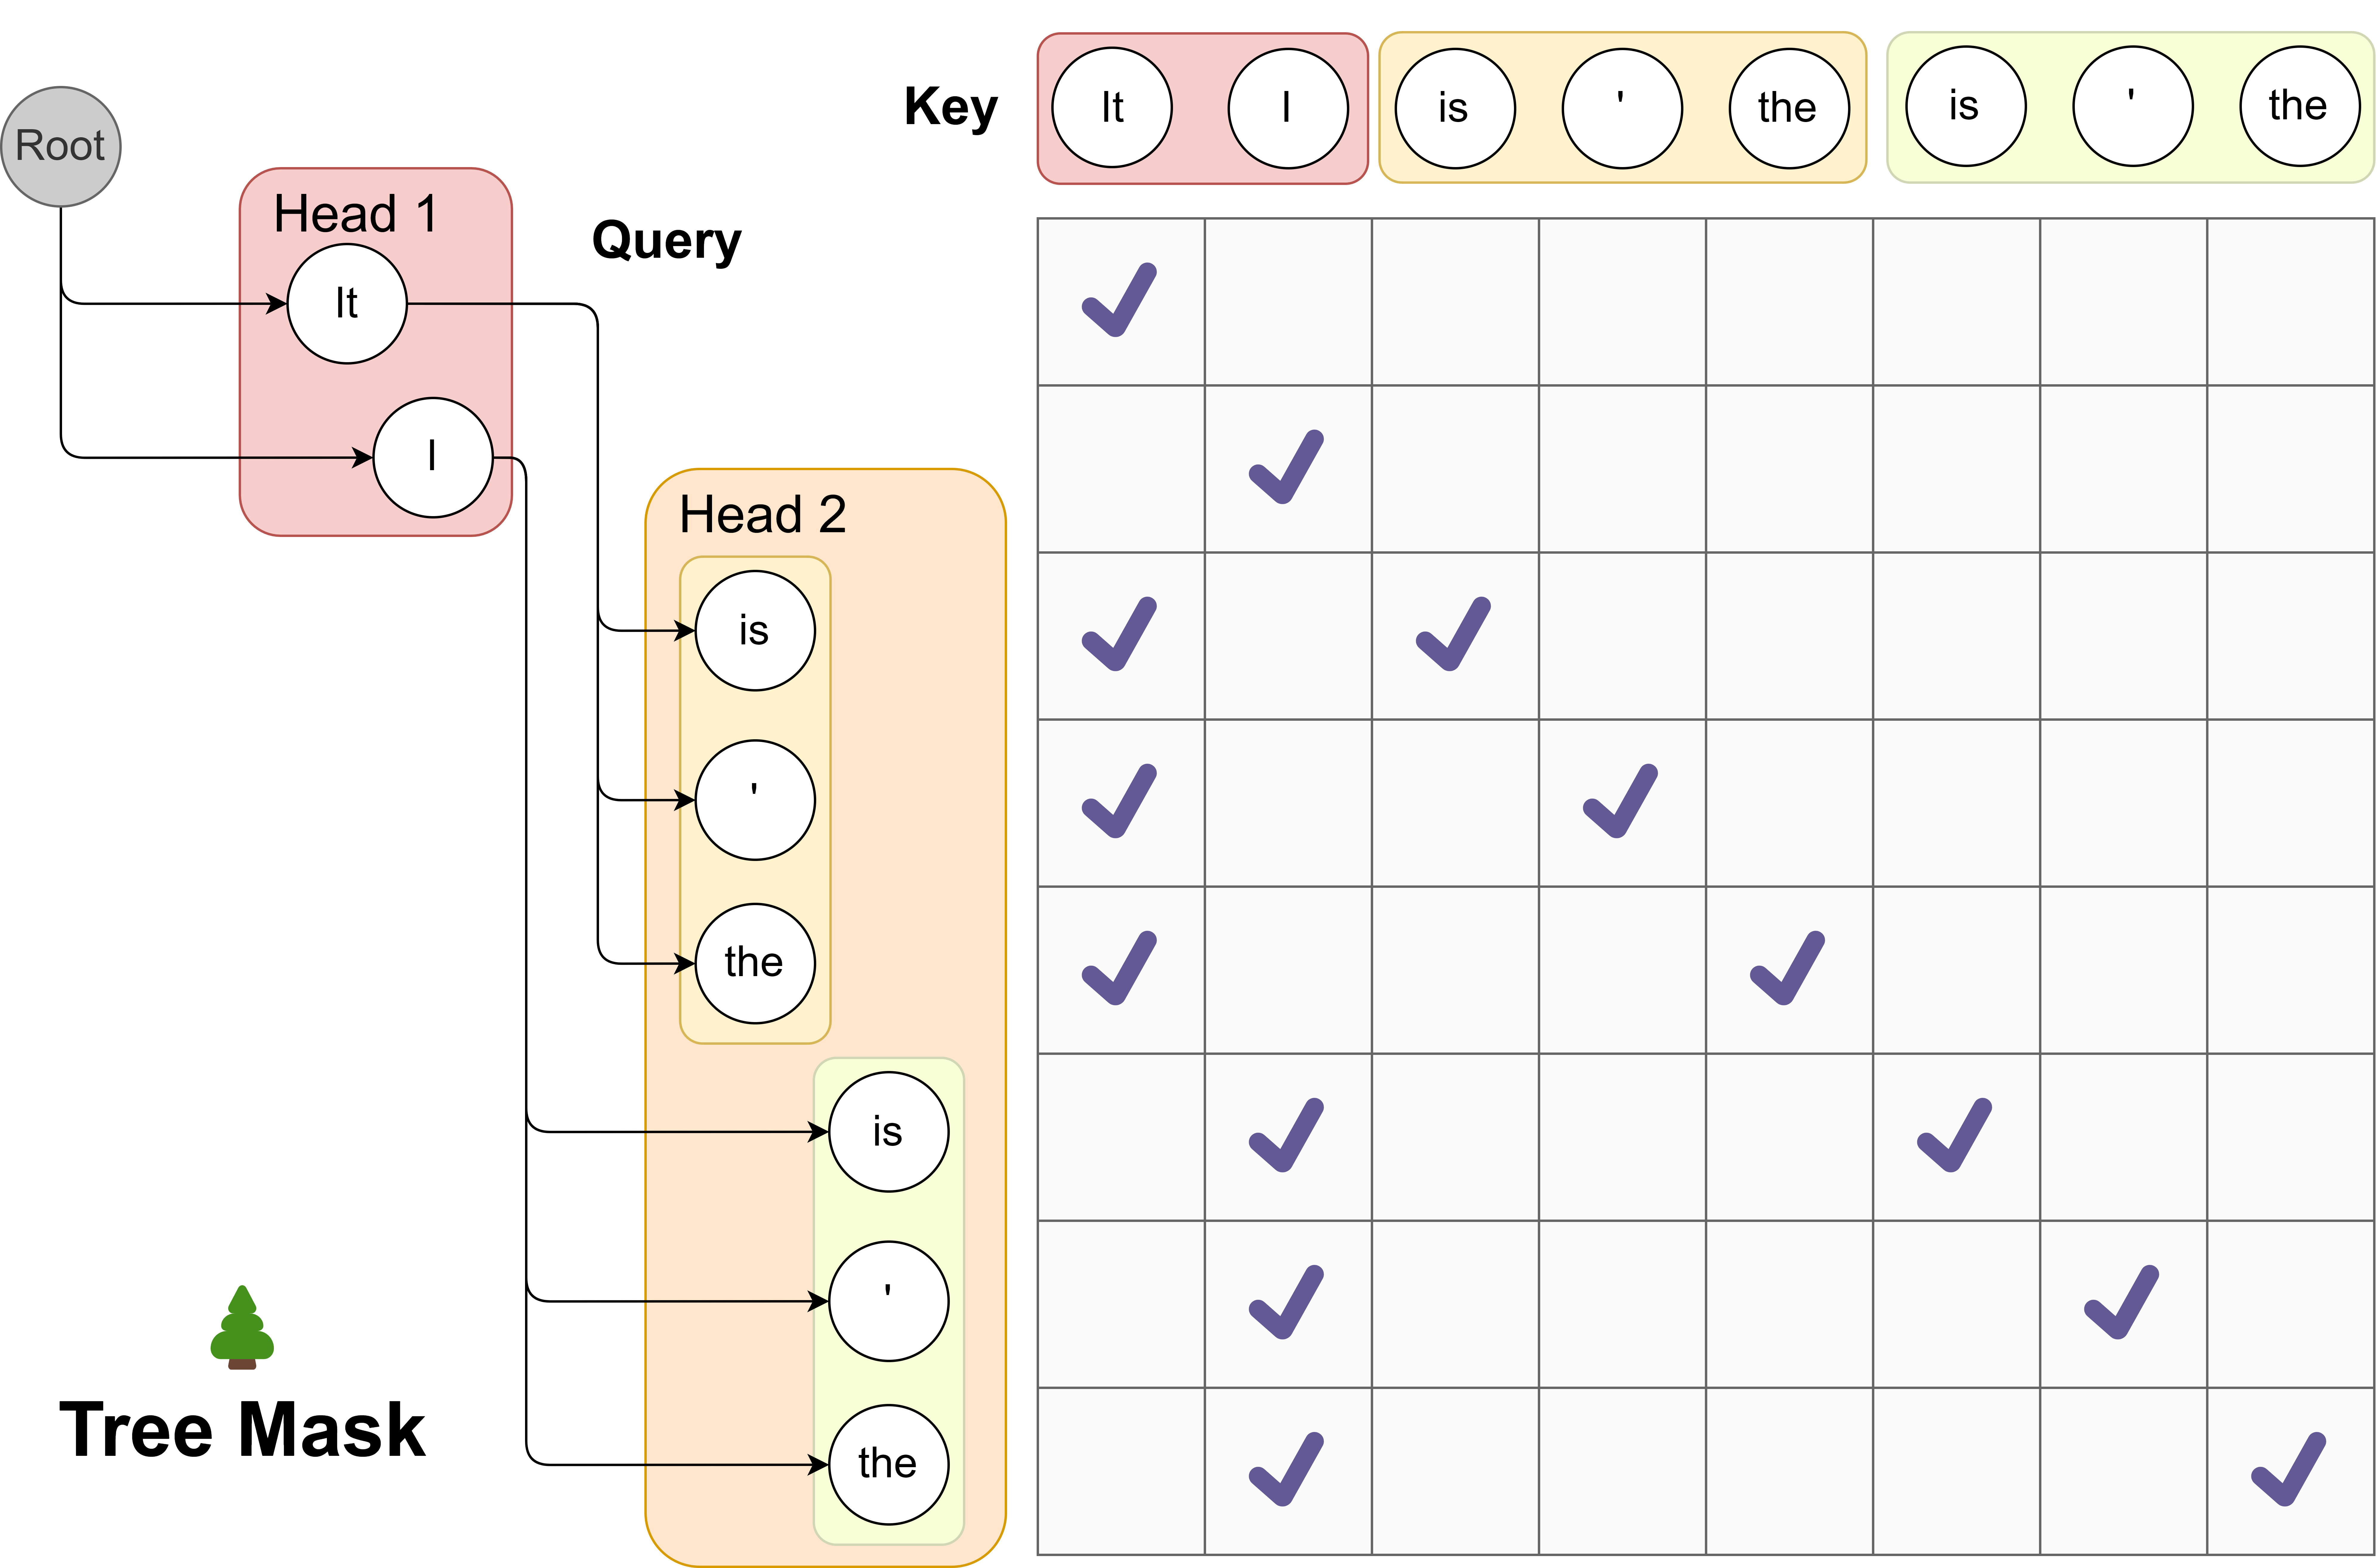
\includegraphics[width=0.45\textwidth]{tree_attention.png}
    \caption{
    We demonstrates the use of tree attention to process multiple candidates concurrently. As exemplified, the top-2 predictions from the first \ours head and the top-3 from the second result in a total of $2\times3=6$ candidates. Each of these candidates corresponds to a distinct branch within the tree structure. To guarantee that each token only accesses its predecessors, we devise an attention mask that exclusively permits attention flow from the current token back to its antecedent tokens. The positional indices for positional encoding are adjusted in line with this structure.}
    \label{fig:tree_attention}
\end{figure}
This attention mechanism diverges from the traditional causal attention paradigm. Within this framework, only tokens from the same continuation are regarded as historical data. Drawing inspiration from the concept of embedding graph structures into attention as proposed in the graph neural network domain~\citep{ying2021transformers}, we incorporate the tree structure into our attention mask, visualized in Figure~\ref{fig:tree_attention}. Remarkably, similar ideas have also been explored in independent works like \citet{miao2023specinfer,spector2023accelerating}, where they follow a bottom-up approach and construct the tree by merging multiple candidates generated by a draft model. In our method, we instead take a top-down approach to build the tree thanks to the structure of candidates generated by \ours heads. For a given $k$-th head, its top-$s_k$ predictions serve as the basis for candidate formation, where $s_k$ is a designated hyperparameter. These candidates are established by determining the Cartesian product of the top-$s_k$ predictions from each head. For instance, in Figure~\ref{fig:tree_attention}, with $s_1=2$ and $s_2=3$, each first head prediction can be succeeded by any prediction from the second head. This leads to a tree structure where $s_k$ branches exist at the $k$-th level (considering a virtual root as the $0$-level, in practice, this $0$-level is for the prediction of the language model head of the original model, which can be sampled independently). Within this tree, only a token's predecessors are seen as historical context, and our attention mask ensures that the attention is only applied on a token's predecessors. By employing this mask and properly setting the positional indices for positional encoding, we can process numerous candidates simultaneously without the need to expand the batch size. The cumulative number of new tokens is calculated as $\sum_{k=1}^K \prod_{i=1}^k s_i$.

In this section, we demonstrate the most simple and regular way to construct the tree structure by taking the Cartesian product. However, it is possible to construct the tree structure in a more sophisticated way and exploit the unbalanced accuracy of different top predictions of different heads. We will discuss this in Section~\ref{sec:optimized_tree_construction}.
\subsection{Training Strategies}
\label{sec:training_recipe}
At the most basic level, we can train \ours heads by freezing the backbone model and fine-tuning \ours heads. However, training the backbone in conjunction with the \ours heads can significantly enhance the accuracy of the \ours heads. Depending on the computational resources and the specific reqirements of the use case, we propose two levels of training strategies for \ours heads.

In this section, we assume the availability of a training dataset that aligns with the target model’s output distribution. This could be the dataset used for Supervised Fine-Tuning (SFT) of the target model. We will discuss eliminating the need for such a dataset using a self-distillation approach in Section~\ref{sec:self_distillation}.
\subsubsection{\ours-1: Frozen Backbone}
\label{sec:frozen_backbone}
To train \ours heads with a frozen backbone model, we can use the cross-entropy loss between the prediction of \ours heads and the ground truth. Specifically, given the ground truth token $y_{t+k+1}$ at position $t+k+1$, the loss for the $k$-th head is $\mathcal{L}_k = -\log p_t^{(k)}(y_{t+k+1})$ where $p_t^{(k)}(y)$ denotes the probability of token $y$ predicted by the $k$-th head. We also observe that $\mathcal{L}_k$ is larger when $k$ is larger, which is reasonable since the prediction of the $k$-th head is more uncertain when $k$ is larger. Therefore, we can add a weight $\lambda_k$ to $\mathcal{L}_k$ to balance the loss of different heads. And the total \ours loss is:
\begin{align}
    \label{eq:loss_medusa_1}
    \mathcal{L}_{\text{\ours-1}} = \sum_{k=1}^K -\lambda_k\log p_t^{(k)}(y_{t+k+1}).
\end{align}

In practice, we set $\lambda_k$ as the $k$-th power of a constant like $0.8$. Since we only use the backbone model for providing the hidden states, we can use a quantized version of the backbone model to reduce the memory consumption. This introduces a more democratized way to accelerate LLM inference, as with the quantization, \ours can be trained for a large model on a single consumer GPU similar to QLoRA~\citep{dettmers2023qlora}. The training only takes a few hours (e.g., 5 hours for \ours-1 on Vicuna 7B model with a single NVIDIA A100 PCIE GPU to train on 60k ShareGPT samples).
\subsubsection{\ours-2: Joint Training}
\label{sec:joint_training}
To further improve the accuracy of \ours heads, we can train \ours heads together with the backbone model. However, this requires a special training recipe to preserve the backbone model's next-token prediction capability and output quality. To achieve this, we propose three strategies:
\begin{itemize}
    \item \textbf{Combined loss}: To keep the backbone model's next-token prediction capability, we need to add the cross-entropy loss of the backbone model $\mathcal{L}_{\text{LM}}=-\log p_t^{(0)}(y_{t+1})$ to the \ours loss. We also add a weight $\lambda_0$ to balance the loss of the backbone model and the \ours heads. Therefore, the total loss is:
    \begin{align}
        \label{eq:loss_medusa_2}
        \mathcal{L}_{\text{\ours-2}} = \mathcal{L}_{\text{LM}} + \lambda_0\mathcal{L}_{\text{\ours-1}}.
    \end{align}
    \item \textbf{Differential learning rates}: Since the backbone model is already well-trained and the \ours heads need more training, we can use separate learning rates for them to enable faster convergence of \ours heads while preserving the backbone model's capability.
    \item \textbf{Heads warmup}: Noticing that at the beginning of training, the \ours heads have a large loss, which leads to a large gradient and may distort the backbone model's parameters. Following the idea from \citet{kumar2022finetuning}, we can employ a two-stage training process. In the first stage, we only train the \ours heads as \ours-1. In the second stage, we train the backbone model and \ours heads together with a warmup strategy. Specifically, we first train the backbone model for a few epochs, then train the \ours heads together with the backbone model. Besides this simple strategy, we can also use a more sophisticated warmup strategy by gradually increasing the weight $\lambda_0$ of the backbone model's loss. We find both strategies work well in practice.
\end{itemize}
Putting these strategies together, we can train \ours heads together with the backbone model without hurting the backbone model's capability. Moreover, this recipe can be applied together with Supervised Fine-Tuning (SFT), enabling us to get a model with native \ours support.
\subsubsection{How to Select the Number of Heads}
Empirically, we found that five heads are sufficient at most. Therefore, we recommend training with five heads and referring to the strategy described in Section~\ref{sec:optimized_tree_construction} to determine the optimal configuration of the tree attention. With optimized tree attention, sometimes three or four heads may be enough for inference. In this case, we can ignore the redundant heads without overhead.

\subsection{Extensions}
\subsubsection{Typical Acceptance}
\label{sec:typical_acceptance}
In speculative decoding papers~\citep{leviathan2022fast,chen2023accelerating}, authors employ rejection sampling to yield diverse outputs that align with the distribution of the original model. However, subsequent implementations~\citep{gante2023assisted,spector2023accelerating} reveal that this sampling strategy results in diminished efficiency as the sampling temperature increases. Intuitively, this can be comprehended in the extreme instance where the draft model is the same as the original one\textcolor{black}{:} 
Using greedy decoding, all output of the draft model will be accepted, therefore maximizing the efficiency. 
Conversely, rejection sampling introduces extra overhead, as the draft model and the original model are sampled independently. Even if their distributions align perfectly, the output of the draft model may still be rejected.

However, in real-world scenarios, sampling from language models is often employed to generate diverse responses, and the temperature parameter is used merely to modulate the ``creativity'' of the response. Therefore, higher temperatures should result in more opportunities for the original model to accept the draft model's output. We ascertain that it is typically unnecessary to match the distribution of the original model. Thus, we propose employing a \emph{typical acceptance} scheme to select plausible candidates rather than using rejection sampling. This approach draws inspiration from truncation sampling studies~\citep{hewitt2022truncation} (refer to \textcolor{black}{Appendix}~\ref{sec:related_work} for an in-depth explanation). Our objective is to choose candidates that are \emph{typical}, meaning they are not exceedingly improbable to be produced by the original model. We use the prediction probability from the \emph{original model} as a natural gauge for this and establish a threshold based on the prediction distribution to determine acceptance. Specifically, given $x_1, x_2, \cdots, x_n$ as context, when evaluating the candidate sequence \textcolor{black}{$(x_{n+1}, x_{n+2}, \cdots, x_{n+K+1})$ }(composed by top predictions of the original language model head and \ours heads), we consider the condition
\begin{align*}
p_{\text{original}}(x_{n+k}|x_1, x_2, \cdots, x_{n+k-1}) > \\\min\rbr{\epsilon, \delta\exp\rbr{-H(p_{\text{original}}(\cdot|x_1, x_2, \cdots, x_{n+k-1}))}},
\end{align*}
where $H(\cdot)$ denotes the entropy function, and $\epsilon, \delta$ are \textcolor{black}{the hard threshold and the entropy-dependent
threshold respectively}. This criterion is adapted from \citet{hewitt2022truncation} and rests on two observations: (1) tokens with relatively high probability are meaningful, and (2) when the distribution's entropy is high, various continuations may be deemed reasonable. During decoding, every candidate is evaluated using this criterion, and a \emph{prefix} of the candidate is accepted if it satisfies the condition. To guarantee the generation of at least one token at each step, we apply \emph{greedy decoding} for the first token and \emph{unconditionally} accept it while employing typical acceptance for subsequent tokens. The final prediction for the current step is determined by the \emph{longest accepted prefix} among all candidates.

Examining this scheme leads to several insights. Firstly, when the temperature is set to $0$, it reverts to greedy decoding, as only the most probable token possesses non-zero probability. As the temperature surpasses $0$, the outcome of greedy decoding will consistently be accepted with appropriate $\epsilon, \delta$, since those tokens have the maximum probability, yielding maximal speedup. Likewise, in general scenarios, an increased temperature will correspondingly result in longer accepted sequences, as corroborated by our experimental findings.

Empirically, we verify that typical acceptance can achieve a better speedup while maintaining a similar \textcolor{black}{generation quality} as shown in Figure~\ref{fig:threshold_ablation}.
\subsubsection{Self-Distillation}
\label{sec:self_distillation}
In Section~\ref{sec:training_recipe}, we assume the existence of a training dataset that matches the target model's output distribution. However, this is not always the case. For example, the model owners may only release the model without the training data, or the model may have gone through a Reinforcement Learning with Human Feedback (RLHF) procedure, which makes the output distribution of the model different from the training dataset. To tackle this issue, we propose an automated self-distillation pipeline to use the model itself to generate the training dataset for \ours heads, which matches the output distribution of the model.

The dataset generation process is straightforward. We first take a public seed dataset from a domain similar to the target model; for example, using the ShareGPT~\citep{sharegpt2023} dataset for chat models. Then, we simply take the prompts from the dataset and ask the model to reply to the prompts. In order to obtain multi-turn conversation samples, we can sequentially feed the prompts from the seed dataset to the model. Or, for models like Zephyr 7B~\citep{tunstall2023zephyr}, which are trained on both roles of the conversation, they have the ability to self-talk, and we can simply feed the first prompt and let the model generate multiple rounds of conversation.

For \ours-1, this dataset is sufficient for training \ours heads. However, for \ours-2, we observe that solely using this dataset for training the backbone and \ours heads usually leads to a lower generation quality. In fact, even without training \ours heads, training the backbone model with this dataset will lead to performance degradation. This suggests that we also need to use the original model's probability prediction instead of using the ground truth token as the label for the backbone model, similar to classic knowledge distillation works~\citep{kim2016sequencelevel}. Concretely, the loss for the backbone model is:
\begin{align*}
    \mathcal{L}_{\text{LM-distill}} = KL(p_{\text{original},t}^{(0)}||p_t^{(0)}),
\end{align*}
where $p_{\text{original},t}^{(0)}$ denotes the probability distribution of the original model's prediction at position $t$.

However, naively, to obtain the original model's probability prediction, we need to maintain two models during training, increasing the memory requirements. To further alleviate this issue, we propose a simple yet effective way to exploit the self-distillation setup. We can use a parameter-efficient adapter like LoRA~\citep{hu2021lora} for fine-tuning the backbone model. In this way, the original model is simply the model with the adapter turned off. Therefore, the distillation does not require additional memory consumption. Together, this self-distillation pipeline can be used to train \ours-2 without hurting the backbone model's capability and introduce almost no additional memory consumption. Lastly, one tip about using self-distillation is that it is preferable to use LoRA without quantization in this case, otherwise, the teacher model will be the quantized model, which may lead to a lower generation quality.

\subsubsection{Searching for the Optimized Tree Construction}
\label{sec:optimized_tree_construction}
In Section~\ref{sec:tree_attention}, we present the simplest way to construct the tree structure by taking the Cartesian product. However, with a fixed budget for the number of total nodes in the tree, a regular tree structure may not be the best choice. Intuitively, those candidates composed of the top predictions of different heads may have different accuracies. Therefore, we can leverage an estimation of the accuracy to construct the tree structure.

Specifically, we can use a calibration dataset and calculate the accuracies of the top predictions of different heads. Let $a_k^{(i)}$ denote the accuracy of the $i$-th top prediction of the $k$-th head\footnote{Here, the accuracy is defined for the single top $i$-th token, i.e., this accuracy is equal to top-$i$ accuracy minus top-$(i-1)$ accuracy.}. Assuming the accuracies are independent, we can estimate the accuracy of a candidate sequence composed by the top $\sbr{i_1, i_2, \cdots, i_k}$ predictions of different heads as $\prod_{j=1}^k a_j^{(i_j)}$. Let $I$ denote the set of all possible combinations of $\sbr{i_1, i_2, \cdots, i_k}$ and each element of $I$ can be mapped to a node of the tree (not only leaf nodes but all nodes are included). Then, the expectation of the acceptance length of a candidate sequence is:
\begin{align*}
    \sum_{\sbr{i_1, i_2, \cdots, i_k}\in I}\prod_{j=1}^k a_j^{(i_j)}.
\end{align*}
Thinking about building a tree by adding nodes one by one, the contribution of a new node to the expectation is exactly the accuracy associated with the node. Therefore, we can greedily add nodes to the tree by choosing the node that is connected to the current tree and has the highest accuracy. This process can be repeated until the total number of nodes reaches the desired number. In this way, we can construct a tree that maximizes the expectation of the acceptance length. Further details can be found in Appendix~\ref{appendix:sparse_tree}.


\vspace{-0.2cm}
\section{Experiments Details}
\label{sec:exp}

\vspace{-0.2cm}
\subsection{Roadmap Insights on FFHQ-256\texorpdfstring{~\cite{sg1}}{}}
\label{sub:arc-experiments}
\vspace{-0.1cm}
As per Table~\ref{tab:roadmap}, Config A (vanilla StyleGAN2) achieves an FID of 7.52 using the official implementation on FFHQ-256. Config B with all tricks removed achieves an FID of 12.46---performance drops as expected. 
Config C, with a well-behaved loss, achieves an FID of 11.65. But, now training is sufficiently stable to improve the architecture.

Config D, which improves $G$ and $D$ based on the classic ResNet and ConvNeXt findings, achieves an FID of 9.95. The output skips of the StyleGAN2 generator are no longer useful given our new architecture; including them produces a worse FID of 10.17. Karras~\etal find that the benefit of output skips is mostly related to gradient magnitude dynamics~\cite{sg3}, and this has been addressed by our ResNet architecture. For StyleGAN2, Karras~\etal conclude that a ResNet architecture is harmful to $G$~\cite{sg2}, but this is not true in our case as their ResNet implementation is considerably different from ours: 1) Karras~\etal use one 3-3 residual block for each resolution stage, while we have a separate transition layer and two 1-3-1 residual blocks; 2) i.3) and i.4) are violated as they do not have a linear residual block~\cite{mobnet} and the transition layer is placed on the skip branch of the residual block rather than the stem; 3) the essential principle of ResNet~\cite{resnet}---identity mapping~\cite{resnet2}---is violated as Karras~\etal divide the output of the residual block by $\sqrt{2}$ to avoid variance explosion due to the absence of a proper initialization scheme.

For Config E, we conduct two experiments that ablate i.\ref{item:i1} (increased width with depthwise conv.) and i.\ref{item:i2} (an inverted bottleneck). We add GroupedConv and reduce the bottleneck compression ratio to two given the same model size. Each bottleneck is now 1.5$\times$ the width of Config A, and the FID drops to 7.51, surpassing the performance of StyleGAN2. By inverting the stem and the bottleneck dimensions to enhance the capacity of GroupedConv, our final model achieves an FID of 7.05, exceeding StyleGAN2.


\begin{wraptable}[12]{r}{6.5cm}
\vspace{-1.25cm}
\centering
\caption{StackedMNIST 1000-mode coverage.}
% Our model outperforms other GANs in terms of $D_\text{KL}$, indicating that we are better able to recover the distribution.}
\vspace{-0.4cm}
\resizebox{0.8\linewidth}{!}{
\begin{tblr}{
  cell{2}{2} = {c},
  cell{2}{3} = {c},
  cell{3}{2} = {c},
  cell{3}{3} = {c},
  cell{4}{2} = {c},
  cell{4}{3} = {c},
  cell{5}{2} = {c},
  cell{5}{3} = {c},
  cell{6}{2} = {c},
  cell{6}{3} = {c},
  cell{7}{2} = {c},
  cell{7}{3} = {c},
  cell{8}{2} = {c},
  cell{8}{3} = {c},
  cell{9}{2} = {c},
  cell{9}{3} = {c},
  cell{10}{2} = {c},
  cell{10}{3} = {c},
  cell{11}{2} = {c},
  cell{11}{3} = {c},
  cell{12}{2} = {c},
  cell{12}{3} = {c},
  hline{2,12} = {1-3}{},
}
Model     & \# modes$\uparrow$ & $D_\text{KL}$$\downarrow$            &  \\
DCGAN~\cite{dcgan}     & 99            & 3.40\phantom{0}&  \\
VEEGAN~\cite{srivastava2017veegan}    & 150           & 2.95\phantom{0}&  \\
WGAN-GP~\cite{wgan-gp}& 959           & 0.73\phantom{0}&  \\
PacGAN~\cite{pacgan}    & 992           & 0.28\phantom{0}&  \\
StyleGAN2~\cite{sg2} & 940           & 0.42\phantom{0}&  \\
PresGAN~\cite{presgan}   & \textbf{1000} & 0.12\phantom{0}&  \\
Adv. DSM~\cite{advsm}  & \textbf{1000} & 1.49\phantom{0}&  \\
VAEBM~\cite{vaebm}     & \textbf{1000} & 0.087          &  \\
DDGAN~\cite{ddgan}     & \textbf{1000} & 0.071          &  \\
MEG~\cite{meg}       & \textbf{1000} & 0.031          &  \\
Ours---Config E     & \textbf{1000} & \textbf{0.029} &  
\end{tblr}
}
\label{tab:stackedmnist}
\end{wraptable}%

\subsection{Mode Recovery --- StackedMNIST\texorpdfstring{~\cite{metz2016unrolled}}{}} 
\vspace{-0.1cm}
We repeat the earlier experiment in 1000-mode convergence on StackedMNIST (unconditional generation), but this time with our updated architecture and with comparisons to SOTA GANs and likelihood-based methods (Tab.~\ref{tab:stackedmnist}, Fig.~\ref{fig:stacked-mnist}). 
One advantage brought up of likelihood-based models such as diffusion over GANs is that they achieve mode coverage~\cite{adm}. We find that most GANs struggle to find all modes. But, PresGAN~\cite{presgan}, DDGAN~\cite{ddgan}, and our approach are successful. Further, our method outperforms all other tested GAN models in term of KL divergence.

\subsection{FID --- FFHQ-256\texorpdfstring{~\cite{sg1}}{} (Optimized)}
\vspace{-0.1cm}
We train Config E model until convergence and with optimized hyperparameters and training schedule on FFHQ at 256$\times$256 (unconditional generation) (Tab.~\ref{tab:ffhq256}, Figs.~\ref{fig:ffhq-256-teaser} and~\ref{fig:ffhq-256}). 
Please see our supplemental material for training details.
%The hyperparameters and schedule are listed in the supplemental material. 
Our model outperforms existing StyleGAN methods, plus four more recent diffusion-based methods. On this common dataset experimental setting, many methods (not listed here) use the bCR~\cite{zhao2021improved} trick---this has only been shown to improve performance on FFHQ-256 (not even at different resolutions of FFHQ)~\cite{zhao2021improved, zhang2022styleswin}. We do not use this trick. 
% no such tricks in our method.
% JT Try to minimize embellishment...
% This is particularly impressive given the fact that the dataset FFHQ was designed for StyleGAN~\cite{sg1} and the StyleGAN series of models were optimized with this specific dataset in mind.
% to achieve this performance.

\subsection{FID --- FFHQ-64\texorpdfstring{~\cite{edm}}{}}
\vspace{-0.1cm}
To compare with EDM~\cite{edm} directly, we evaluate our model on FFHQ at 64$\times$64 resolution. For this, we remove the two highest resolution stages of our 256$\times$256 model, resulting in a generator that is less than half the number of parameters as EDM. Despite this, our model outperforms EDM on this dataset and needs one function evaluation only (Tab.~\ref{tab:ffhq64}).

\begin{figure}
\begin{floatrow}
    %\hspace{-0.75cm}%
    \capbtabbox{%
        \centering
        \resizebox{\linewidth}{!}{
        \begin{tblr}{
          column{2,3} = {r},
          cell{1}{2} = {c},
          cell{1}{3} = {c},
          hline{2,5,9,10} = {-}{},
        }
        Model       & NFE$\downarrow$ & FID$\downarrow$  \\
        StyleGAN2~\cite{sg2}   & 1               & 3.78 \\
        StyleGAN3-T~\cite{sg3} & 1               & 4.81 \\
        StyleGAN3-R~\cite{sg3} & 1               & 3.92 \\
        LDM~\cite{rombach2022high} & 200               & 4.98\\
        ADM (DDIM)~\cite{adm,compdiff} & 500               & 8.41\\
        ADM (DPM-Solver)~\cite{adm,compdiff} & 500               & 8.40\\
        Diffusion Autoencoder~\cite{diffae,compdiff} & 500               & 5.81\\
        Ours---Config E  & 1               & 2.75 \\
        \emph{With ImageNet feature leakage~\cite{kynkaanniemi2022role}:} & & \\
        PolyINR*~\cite{singh2023polynomial} & 1               & 2.72 \\
        StyleGAN-XL*~\cite{sgxl} & 1               & 2.19 \\
        StyleSAN-XL*~\cite{takida2024san} & 1               & 1.68 \\
        \end{tblr}
        }
    }{%
        \caption{
        \label{tab:ffhq256}FFHQ-256. * denotes models that leak ImageNet features.}
    }
    %
    \capbtabbox{%
        \centering
        \resizebox{0.85\linewidth}{!}{
        \begin{tblr}{
          column{2} = {r},
          column{3} = {r},
          hline{2,5,8} = {-}{},
        }
        Model         & NFE$\downarrow$ & FID$\downarrow$ \\
        StyleGAN2~\cite{sg2,anycostgan}     & 1               & 3.32            \\
        MSG-GAN~\cite{karnewar2020msg,anycostgan}       & 1               & 2.7             \\
        Anycost GAN~\cite{anycostgan}   & 1               & 2.52            \\
        VE~\cite{sde,edm}            & 79              & 25.95           \\
        VP~\cite{sde,edm}            & 79              & 3.39            \\
        EDM~\cite{edm}           & 79              & 2.39            \\
        Ours—Config E & 1               & 1.95 \\
        \end{tblr}
        }
    }{%
        \caption{\label{tab:ffhq64}FFHQ-64.}
    }
\end{floatrow}
\vspace{-0.25cm}
\end{figure}


% \begin{figure}
% \begin{floatrow}
%     \capbtabbox{%
%         \centering
%         \resizebox{0.8\linewidth}{!}{
%         \begin{tblr}{
%           column{2,3} = {r},
%           cell{1}{2} = {c},
%           cell{1}{3} = {c},
%           hline{2,9,13} = {-}{},
%         }
%         Model               & NFE$\downarrow$ & FID$\downarrow$ \\
%         BigGAN~\cite{biggan}              & 1               & 14.73 \\
%         TransGAN~\cite{trans}            & 1               & 9.26 \\
%         ViTGAN~\cite{vitgan}              & 1               & 6.66 \\
%         DDGAN~\cite{ddgan}               & 4               & 3.75 \\
%         Diffusion StyleGAN2~\cite{diffusiongan} & 1               & 3.19 \\
%         StyleGAN2 + ADA~\cite{sg2ada}     & 1               & 2.42 \\
%         StyleGAN3-R + ADA~\cite{sg3,studio}   & 1               & 10.83 \\
%         DDPM~\cite{ddpm}               & 1000            & 3.21 \\
%         DDIM~\cite{ddim}                & 50             & 4.67 \\
%         VE~\cite{sde,edm}                  & 35              & 3.11 \\
%         VP~\cite{sde,edm}                  & 35              & 2.48 \\
%         Ours---Config E     & 1               & 1.96 \\
%         \hline
%         \emph{With ImageNet feature leakage~\cite{kynkaanniemi2022role}:} & & \\
%         StyleGAN-XL*~\cite{sgxl}       & 1               & 1.85 \\
%         \end{tblr}
%         }
%     }{%
%         \caption{\label{tab:cifar10}CIFAR-10.}
%     }
%         % \begin{tblr}{
%         %   column{2,3} = {r},
%         %   cell{1}{2}{3} = {},
%         %   hline{2,9,13} = {-}{},
%         % }
%         % Model               & FID$\downarrow$ & Params          \\
%         % BigGAN~\cite{biggan}              & 14.73  & --       \\
%         % TransGAN~\cite{trans}            & 9.26 & --         \\
%         % ViTGAN~\cite{vitgan}              & 6.66 & --         \\
%         % DDGAN~\cite{ddgan}               & 3.75 & --         \\
%         % Diffusion StyleGAN2 & 3.19 & 40.1M           \\
%         % StyleGAN2 + ADA     & 2.42 & 40.1M          \\
%         % StyleGAN3-R + ADA   & 10.83 & 40.1M        \\
%         % DDPM               & 3.21 & 35.2M         \\
%         % DDIM                & 4.67 & --         \\
%         % VE~\cite{edm}                  & 3.11 & 61.8M        \\
%         % VP~\cite{edm}                  & 2.48 & 61.8M         \\
%         % Ours---Config E     & \textbf{1.99}  & 43.0M \\
%         % StyleGAN-XL*~\cite{sgxl}       & 	1.85 & 140.0M \\
%         % \end{tblr}
        
%     %     }
%     % }{%
%     %     \caption{\label{tab:cifar10}CIFAR-10.}
%     % }%
%     %\hspace{-0.75cm}%
%     %\hspace{-0.5cm}%
% \end{floatrow}
% \end{figure}

\subsection{FID --- CIFAR-10~\cite{krizhevsky2009learning}} \vspace{-0.1cm}

\begin{wraptable}[14]{r}{6.5cm}
\vspace{-0.75cm}
\centering
\caption{\label{tab:cifar10}CIFAR-10 performance.}
\vspace{-0.4cm}
\resizebox{0.9\linewidth}{!}{
    \begin{tblr}{
          column{2,3} = {r},
          cell{1}{2} = {c},
          cell{1}{3} = {c},
          hline{2,9,13} = {-}{},
        }
        Model               & NFE$\downarrow$ & FID$\downarrow$ \\
        BigGAN~\cite{biggan}              & 1               & 14.73 \\
        TransGAN~\cite{trans}            & 1               & 9.26 \\
        ViTGAN~\cite{vitgan}              & 1               & 6.66 \\
        DDGAN~\cite{ddgan}               & 4               & 3.75 \\
        Diffusion StyleGAN2~\cite{diffusiongan} & 1               & 3.19 \\
        StyleGAN2 + ADA~\cite{sg2ada}     & 1               & 2.42 \\
        StyleGAN3-R + ADA~\cite{sg3,studio}   & 1               & 10.83 \\
        DDPM~\cite{ddpm}               & 1000            & 3.21 \\
        DDIM~\cite{ddim}                & 50             & 4.67 \\
        VE~\cite{sde,edm}                  & 35              & 3.11 \\
        VP~\cite{sde,edm}                  & 35              & 2.48 \\
        Ours---Config E     & 1               & 1.96 \\
        \hline
        \emph{With ImageNet feature leakage~\cite{kynkaanniemi2022role}:} & & \\
        StyleGAN-XL*~\cite{sgxl}       & 1               & 1.85 \\
        \end{tblr}
}
\end{wraptable}

We train Config E model until convergence and with optimized hyperparameters and training schedule on CIFAR-10 (conditional generation) (Tab.~\ref{tab:cifar10}, Fig.~\ref{fig:cifar10}). Our method outperforms many other GANs by FID even though the model has relatively small capacity. For instance, StyleGAN-XL~\cite{sgxl} has 18\ M parameters in the generator and 125\ M parameters in the discriminator, while our model has a 40\ M parameters between the generator and discriminator combined (Fig.~\ref{fig:fid-50k-vs-params-cifar-10}). Compared to diffusion models like LDM or ADM, GAN inference is significantly cheaper as it requires only one network function evaluation compared to the tens or hundreds of network function evaluations for diffusion models without distillation. 

\begin{wrapfigure}[12]{r}{6.5cm}
    \vspace{-0.4cm}
    \centering
    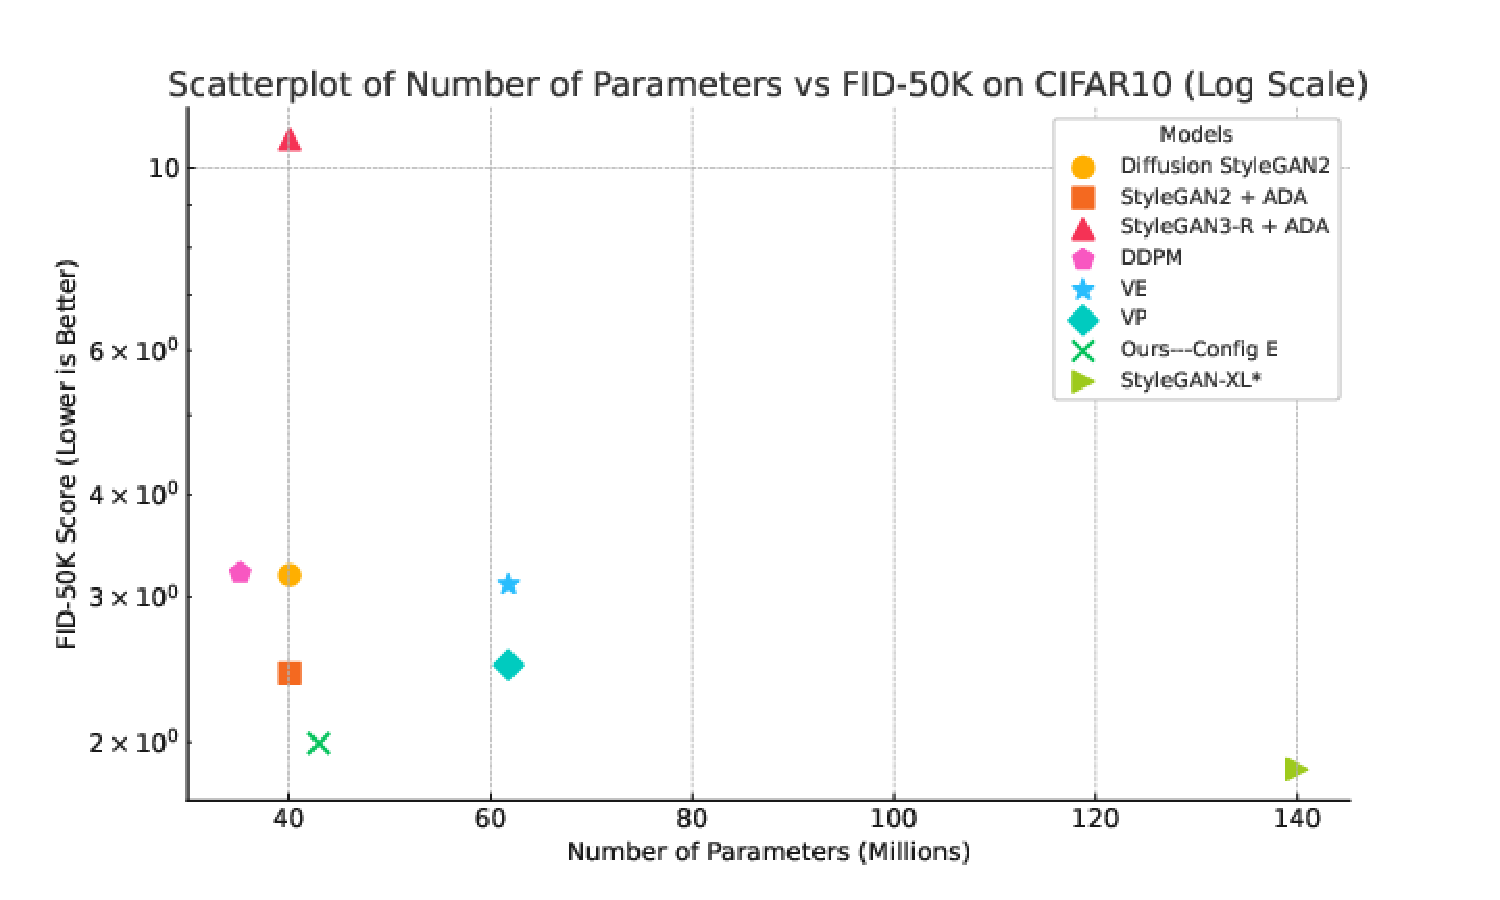
\includegraphics[width=\linewidth,clip,trim={0 0 0 2cm}]{figures/Scatterplot-FID-Parameters-CIFAR10.pdf}
    \caption{Millions of parameters vs.~FID-50K (log scale) on CIFAR-10. Lower is better.}
    \label{fig:fid-50k-vs-params-cifar-10}
\end{wrapfigure}

Many state-of-the-art GANs are derived from Projected GAN~\cite{sauer2021projected}, including StyleGAN-XL~\cite{sgxl} and the concurrent work of StyleSAN-XL~\cite{takida2024san}. These methods use a pre-trained ImageNet classifier in the discriminator. Prior work has shown that a pre-trained ImageNet discriminator can leak ImageNet features into the model~\cite{kynkaanniemi2022role}, causing the model to perform better when evaluating on FID since it relies on a pre-trained ImageNet classifier for the loss. But, this does not improve results in perceptual studies~\cite{kynkaanniemi2022role}. Our model produces its low FID without any ImageNet pre-training.

%\jt{Missing citations here for such methods.}


%\aaron{add NFEs}
%\jt{Which models in our evaluation use this? Any?}

%\jt{What is the second caveat?}

\subsection{FID --- ImageNet-32~\cite{chrabaszcz2017downsampled}}
\label{sec:imagenet32-fid-explain}
We train Config E model until convergence and with optimized hyperparameters and training schedule on ImageNet-32 (conditional generation). We compare against recent GAN models and recent diffusion models in Table~\ref{tab:imagenet32}.
We adjust the number of parameters in the generator of our model to match StyleGAN-XL~\cite{sgxl}'s generator (84M parameters). Specifically, we make the model significantly wider to match. Our method achieves comparable FID despite using a 60\% smaller discriminator (Tab.~\ref{tab:imagenet32}) and despite not using a pre-trained ImageNet classifier.
%, which has been shown to improve FID performance, but not improve results in perceptual studies~\cite{kynkaanniemi2022role}.

\vspace{-0.1cm}
\subsection{FID --- ImageNet-64~\cite{chrabaszcz2017downsampled}}
We evaluate our model on ImageNet-64 to test its scalability. We stack another resolution stage on our ImageNet-32 model, resulting in a generator of 104\ M parameters. This model is nearly 3$\times$ smaller than diffusion-like models~\cite{adm,edm,cm,icm} that rely on the ADM backbone, which contains about 300\ M parameters. Despite the smaller model size and that our model generates samples in one step, it outperforms larger diffusion models with many NFEs on FID (Tab.~\ref{tab:imagenet64}).

\vspace{-0.1cm}
\subsection{Recall}
We evaluate the recall~\cite{precrecall} of our model on each dataset to quantify sample diversity. In general, our model achieves a recall that is similar to or marginally worse than the diffusion model counterpart, yet superior to existing GAN models. For CIFAR-10, the recall of our model peaked at 0.57; as a point of comparison, StyleGAN-XL~\cite{sgxl} has a worse recall of 0.47 despite its lower FID. For FFHQ, we obtain a recall of 0.53 at 64$\times$64 and 0.49 at 256$\times$256, whereas StyleGAN2~\cite{sg2} achieved a recall of 0.43 on FFHQ-256. Our ImageNet-32 model achieved a recall of 0.63; comparable to ADM~\cite{adm}. Our ImageNet-64 model achieved recall 0.59. While this is slightly worse than $\approx$0.63 that many diffusion models achieve, it is better than BigGAN-deep~\cite{biggan} which achieved a recall of 0.48.

\begin{figure}
    \begin{floatrow}
        \capbtabbox{%
        \centering
        \resizebox{0.9\linewidth}{!}{
        \begin{tblr}{
          column{2} = {r},
          column{3} = {r},
          cell{8}{1} = {c=3}{},
          hline{2,7-8} = {-}{},
        }
    Model                                                       & NFE$\downarrow$  & FID$\downarrow$                        \\ 
    DDPM++~\cite{kim2021soft}                  & 1000 & 8.42                                   \\
    VDM~\cite{kingma2021variational}           & 1000 & 7.41                                   \\
    MSGAN~\cite{karnewar2020msg,ning2023input} & 1    & 12.3                                   \\
    ADM~\cite{adm}                             & 1000 & 3.60                                   \\
    DDPM-IP~\cite{ning2023input}               & 1000 & 2.87                                   \\
    Ours—Config E               & 1    & 1.27   \\
    \textit{With ImageNet feature leakage~\cite{kynkaanniemi2022role}:}    \\
    StyleGAN-XL*~\cite{sgxl}                   & 1    & 1.10                                  
    \end{tblr}
        }
    }{%
        \caption{\label{tab:imagenet32}ImageNet-32.}
        % \jt{some are conditional still}}
    }
    %
    \capbtabbox{
        \centering
        \resizebox{0.9\linewidth}{!}{
        \begin{tblr}{
          column{2} = {r},
          column{3} = {r},
          cell{1}{2} = {c},
          cell{1}{3} = {c},
          cell{12}{1} = {c=3}{},
          hline{2-3,11-12} = {-}{},
        }
        Model         & NFE$\downarrow$ & FID$\downarrow$ \\
        BigGAN-deep~\cite{biggan}\phantom{xx}   & 1               & 4.06            \\
        DDPM~\cite{ddpm}          & 250             & 11.0            \\
        DDIM~\cite{ddim}          & 50              & 13.7            \\
        ADM~\cite{adm}           & $^\S$250             & 2.91            \\
        EDM~\cite{edm}           & 79              & 2.23            \\
        CT~\cite{cm}            & 2               & 11.1            \\
        CD~\cite{cm}            & 3               & 4.32            \\
        iCT-deep~\cite{icm}      & 2               & 2.77            \\
        DMD~\cite{dmd}           & 1               & 2.62            \\
        Ours—Config E & 1               & 2.09            \\
        \emph{With ImageNet feature leakage~\cite{kynkaanniemi2022role}:}          &                 &                 \\
        StyleGAN-XL*~\cite{sgxl}   & 1               & 1.52            
        \end{tblr}
        }
    }
    {
        \caption{\label{tab:imagenet64}ImageNet-64.\hspace{-0.1cm} {\small \S:\hspace{-0.05cm}deterministic sampling.}}
    }
    \end{floatrow}
    \vspace{-0.25cm}
\end{figure}


% \begin{table}[ht]
%     \centering
%     \begin{tabular}{lcccccccc}
%         \toprule
%         \textbf{Model} & \textbf{\# Param.} & \textbf{IS $\uparrow$} & \textbf{FID $\downarrow$} & \textbf{Precision $\uparrow$} & \textbf{Recall $\uparrow$} & \textbf{Density $\uparrow$} & \textbf{Coverage $\uparrow$} & \textbf{Inf. (s)} \\
%         \midrule
%         ReACGAN + DiffAug (Ours) [10] & 9.4M & 10.15 & 2.64 & 0.75 & 0.65 & 0.98 & 0.90 & 0.009 \\
%         StyleGAN2-ADA [85] & 20.2M & 10.31 & 2.41 & 0.74 & 0.68 & 1.02 & 0.92 & 0.008 \\
%         StyleGAN2-ADA (Ours) [85] & 20.2M & \textbf{10.53} & 2.31 & 0.75 & 0.69 & 1.04 & 0.93 & 0.008 \\
%         StyleGAN2 + DiffAug + D2D-CE (Ours) [10] & 20.2M & 10.46 & 2.30 & 0.76 & 0.68 & 1.03 & 0.93 & 0.007 \\
%         DDPM [43] & 35.2M & 9.73 & 3.23 & 0.78 & 0.67 & 1.10 & 0.93 & 15.422 \\
%         DDPM++ [44] & 106.6M & 9.90 & 2.49 & 0.78 & 0.69 & 1.12 & 0.94 & 46.697 \\
%         NCSN++ [44] & 107.6M & 10.08 & 2.27 & 0.77 & 0.70 & 1.07 & 0.94 & 99.304 \\
%         LSGM [45] & - & 10.04 & 2.80 & 0.80 & 0.70 & 1.15 & 0.95 & - \\
%         LSGM-ODE [45] & - & 10.07 & \textbf{2.09} & 0.77 & 0.71 & 1.03 & 0.94 & - \\
%         CLD-SGM [47] & - & 9.88 & 2.38 & 0.78 & 0.69 & 1.12 & 0.94 & - \\
%         StyleGAN-XL~ & 18.0M & \textbf{11.03} & \textbf{1.88} & 0.77 & 0.59 & 1.08 & 0.94 & 0.010 \\
%         % BaselineGAN & %10.284011840820312
%         % 10.28
%         % & %1.9925376117527978 
%         % 1.99 & % 0.6899600028991699 
%         % 0.69 &&
%         \bottomrule
%     \end{tabular}
%     \caption{Comparison of various models on CIFAR10 dataset. TODO fix citation}
% \label{tab:cifar10_comparison}
%\end{table}

% \jt{Is the below meant to be a conclusion? Some of these statements are unfounded in the evidence we present so far.}
% \begin{enumerate}

%     \item We demonstrate the ability of our method to recover all modes of training data on Stacked Mnist~\ref{tab:stackedmnist}.
%     \item We beat all methods that do not use bCR (shown to overfit for FFHQ-256~\cite{}) and methods that do not leak imagenet features from a pretrained discriminator~\cite{kynkaanniemi2022role}. If we exclude these two categories of models, we are SOTA across all open source GANs. We also SOTA on a per parameter count basis on multiple GANs.
%     \item We demonstrate SOTA performance on CIFAR-10 image generation at our current parameter count, outperforming all previous GANs except for StyleGAN-XL derived ones with X\% percent of the parameters of these methods. We also do not leak features from ImageNet or use a pretrained discriminator.~\ref{tab:cifar10}. 
%     \item We achieve near SOTA on FFHQ 256 and achieve SOTA for a GAN method without bCR or feature leakage.
%     \item We achieve near state of the art results on Imagenet and achieve Pareto frontier results for total GAN model parameter size.
% \end{enumerate}
% \begin{table}[h]
\centering
\caption{FID on ImageNet-32}
\begin{tabular}{ l c c }
\toprule
Model & \textbf{Year} & FID$\downarrow$ \\
\midrule
% %Real NVP (Dinh et al.) & 2016 & 4.28 \\
% %Glow (Kingma and Dhariwal) & 2018 & 4.09 \\
% %MintNet & 2019 & 4.06 \\
% % Residual Flow & 2019 & 4.01 \\
% % BIVA Maaloe et al. & 2019 & 3.96 \\
% % ANF Huang et al. & 2020 & 3.92 \\
% % NVAE w/ flow & 2020 & 3.92 \\
% % PixelRNN & 2016 & 3.86 \\
% % Flow++ & 2019 & 3.86 \\
% % SPN Menick and Kalchbrenner & 2018 & 3.85 \\
% % Gated PixelCNN & 2016 & 3.83 \\
% % Very Deep VAE & 2020 & 3.8 \\
% % MRCNF & 2021 & 3.77 \\
% % $\delta$-VAE & 2019 & 3.77 \\
% Image Transformer~\cite{parmar2018image} & 2018 & 3.77 \\
% ScoreFlow & 2021 & 3.76 \\
% Reflected Diffusion & 2023 & 3.74 \\
% %Hourglass & 2021 & 3.74 \\
% DenseFlow-74-10 & 2021 & 3.63 \\
% i-DODE & 2023 & 3.43 \\
% MSGAN~\cite{karnewar2020msg} & 2019 & 12.3 \\
% DDPM-IP & 2023 & 2.66 \\
MSGAN~\cite{karnewar2020msg} & 2019 & 12.3 \\
VDM~\cite{kingma2021variational} & 2021 & 7.41 \\
DDPM++~\cite{kim2021soft} & 2021 & 8.42 \\
DDPM-IP~\cite{ning2023input} & 2023 & 2.87 \\
\textbf{Ours} & 2024 & 1.28 \\
StyleGAN-XL~\cite{sauer2022stylegan} & 2022 & \textbf{1.10} \\
\bottomrule
\end{tabular}
\end{table}

% \begin{table}[tO]
%     \centering
%     \begin{tabular}{c|c|c|c}
%          & FID\_50k & Precision & Recall \\
%         StyleGAN &  \\
%         StyleGAN-XL? &
%         Lots of other baselines
%     \end{tabular}
%     \caption{Caption}
%     \label{tab:my_label}
% \end{table}
% \label{sec:exp}
% % cifar10, ffhq, imagenet

% \begin{table}
%     \centering
%     %\caption{Results for CIFAR-10 generation. \aaron{add NFEs}}
%     %\vspace{-2mm}
%     \begin{tblr}{
%       column{2} = {r},
%       cell{1}{2} = {c},
%       hline{2,9,13} = {-}{},
%     }
%     Model               & FID$\downarrow$           \\
%     BigGAN~\cite{biggan}              & 14.73         \\
%     TransGAN~\cite{trans}            & 9.26          \\
%     ViTGAN~\cite{vitgan}              & 6.66          \\
%     DDGAN~\cite{ddgan}               & 3.75          \\
%     Diffusion StyleGAN2 & 3.19          \\
%     StyleGAN2 + ADA     & 2.42          \\
%     StyleGAN3-R + ADA   & 10.83         \\
%     DDPM                & 3.21          \\
%     DDIM                & 4.67          \\
%     VE                  & 3.11          \\
%     VP                  & 2.48          \\
%     Ours---Config E     & \textbf{1.99} 
%     \end{tblr}
%     %\label{tab:cifar10}
%     \caption{Results for CIFAR-10 generation. \aaron{add NFEs}}
%     \label{tab:cifar10}
% \end{table}



%%%%%%%%%%%%%%%%%%%%%%%%%%%%%%%%%%%%%%%%%%%%%%%%%%%%%%%%%%%%%
% Qualitative figures
%%%%%%%%%%%%%%%%%%%%%%%%%%%%%%%%%%%%%%%%%%%%%%%%%%%%%%%%%%%%%

% Variable to control the size of each image
% \begin{figure}
%     \centering
%     \includegraphics{example-image-a}
%     \caption{stacked mnist (qualitative figure) (from powerpoint)}
%     \label{fig:stacked-mnist}
% \end{figure}
% cifar10, ffhq, imagenet

% \noindent\begin{minipage}{.33\textwidth}
% \centering
% \captionof{table}{1000-mode coverage on StackedMNIST.}
% \vspace{-2mm}
% \begin{tblr}{
%   cell{2}{2} = {c},
%   cell{2}{3} = {c},
%   cell{3}{2} = {c},
%   cell{3}{3} = {c},
%   cell{4}{2} = {c},
%   cell{4}{3} = {c},
%   cell{5}{2} = {c},
%   cell{5}{3} = {c},
%   cell{6}{2} = {c},
%   cell{6}{3} = {c},
%   cell{7}{2} = {c},
%   cell{7}{3} = {c},
%   cell{8}{2} = {c},
%   cell{8}{3} = {c},
%   cell{9}{2} = {c},
%   cell{9}{3} = {c},
%   cell{10}{2} = {c},
%   cell{10}{3} = {c},
%   cell{11}{2} = {c},
%   cell{11}{3} = {c},
%   hline{2,11} = {1-3}{},
% }
% Model     & Modes$\uparrow$ & KLD$\downarrow$            &  \\
% DCGAN     & 99            & 3.40\phantom{0}&  \\f
% VEEGAN    & 150           & 2.95\phantom{0}&  \\
% WGAN-GP   & 959           & 0.73\phantom{0}&  \\
% PacGAN    & 992           & 0.28\phantom{0}&  \\
% StyleGAN2 & 940           & 0.42\phantom{0}&  \\
% PresGAN   & \textbf{1000} & 0.12\phantom{0}&  \\
% Adv. DSM  & \textbf{1000} & 1.49\phantom{0}&  \\
% VAEBM     & \textbf{1000} & 0.087          &  \\
% DDGAN     & \textbf{1000} & 0.071          &  \\
% Ours      & \textbf{1000} & \textbf{???} &  
% \end{tblr}
% \label{tab:stackedmnist}
% \end{minipage}%
% \begin{minipage}{.33\textwidth}
% \centering
% \captionof{table}{Results for CIFAR-10 generation.}
% \vspace{-2mm}
% \begin{tblr}{
%   column{2} = {r},
%   cell{1}{2} = {c},
%   hline{2,9,13} = {-}{},
% }
% Model               & FID$\downarrow$           \\
% BigGAN              & 14.73         \\
% TransGAN            & 9.26          \\
% ViTGAN              & 6.66          \\
% DDGAN               & 3.75          \\
% Diffusion StyleGAN2 & 3.19          \\
% StyleGAN2 + ADA     & 2.42          \\
% StyleGAN3-R + ADA   & 10.83         \\
% DDPM                & 3.21          \\
% DDIM                & 4.67          \\
% VE                  & 3.11          \\
% VP                  & 2.48          \\
% Ours                & \textbf{1.99} 
% \end{tblr}
% \label{tab:cifar10}
% \end{minipage}%
% \begin{minipage}{.33\textwidth}
% \centering
% \captionof{table}{Results on FFHQ ($256\times256$).}
% \vspace{-2mm}
% \begin{tblr}{
%   column{2} = {r},
%   cell{1}{2} = {c},
%   hline{2,5} = {-}{},
%   hline{2,9} = {-}{},
% }
% Model       & FID$\downarrow$  \\
% StyleGAN2   & 3.78 \\
% StyleGAN3-T & 4.81 \\
% StyleGAN3-R & 3.92 \\
% LDM & 4.98\\
% ADM (DDIM) & 8.41\\
% ADM (DPM-Solver) & 8.40\\
% Diffusion Autoencoder & 5.81\\
% Ours        & \textbf{2.95} 
% \end{tblr}
% \label{tab:ffhq256}
% \end{minipage}


% \input{tables/cifar10}
% \input{tables/ffhq256}
% \input{tables/MNIST}
\begin{figure}[h!]
    \newlength{\imgsize}
    \setlength{\imgsize}{0.10\linewidth} % Adjust this value to change the size of the images
    
    % New command to include images from a specific directory
    \newcommand{\qualitativeimg}[1]{%
        \includegraphics[width=\imgsize]{figures/qualitative/ffhq-256-000139623/image-#1.jpg}%
    }
    
    \setlength{\tabcolsep}{0pt} % Remove spacing between columns
    \renewcommand{\arraystretch}{0} % Remove spacing between rows
    
    \centering
    \begin{tabular}{cccccccc} % Eight columns
        \qualitativeimg{64} & \qualitativeimg{65} & \qualitativeimg{66} & \qualitativeimg{67} & \qualitativeimg{128} & \qualitativeimg{69} & \qualitativeimg{70} & \qualitativeimg{71} \\
        \qualitativeimg{72} & \qualitativeimg{73} & \qualitativeimg{74} & \qualitativeimg{75} & \qualitativeimg{76} & \qualitativeimg{77} & \qualitativeimg{78} & \qualitativeimg{79} \\
        \qualitativeimg{80} & \qualitativeimg{81} & \qualitativeimg{82} & \qualitativeimg{83} & \qualitativeimg{84} & \qualitativeimg{85} & \qualitativeimg{86} & \qualitativeimg{87} \\
        \qualitativeimg{88} & \qualitativeimg{89} & \qualitativeimg{90} & \qualitativeimg{91} & \qualitativeimg{92} & \qualitativeimg{93} & \qualitativeimg{94} & \qualitativeimg{95} \\
        \qualitativeimg{96} & \qualitativeimg{97} & \qualitativeimg{98} & \qualitativeimg{99} & \qualitativeimg{100} & \qualitativeimg{101} & \qualitativeimg{102} & \qualitativeimg{103} \\
        \qualitativeimg{104} & \qualitativeimg{105} & \qualitativeimg{106} & \qualitativeimg{107} & \qualitativeimg{108} & \qualitativeimg{109} & \qualitativeimg{110} & \qualitativeimg{111} \\
        \qualitativeimg{112} & \qualitativeimg{113} & \qualitativeimg{114} & \qualitativeimg{115} & \qualitativeimg{116} & \qualitativeimg{117} & \qualitativeimg{118} & \qualitativeimg{119} \\
        \qualitativeimg{120} & \qualitativeimg{121} & \qualitativeimg{122} & \qualitativeimg{123} & \qualitativeimg{124} & \qualitativeimg{125} & \qualitativeimg{126} & \qualitativeimg{127} \\
    \end{tabular}
    \caption{Qualitative examples of sample generation from our Config E on FFHQ-256.}
    \label{fig:ffhq-256-teaser}
\end{figure}


\vspace{-7pt}
\section{Conclusion}
\vspace{-8pt}
In this work, we study Continual Self-Supervised Learning (CSSL), the problem of learning a set of tasks without labels continually. We make two important contributions for the SSL and CL communities: (i) we present \name{}, a simple and effective framework for CSSL that shows how SSL methods and losses can be seamlessly reused to learn continually, and (ii) we perform a comprehensive analysis of CSSL, leading to the emergence of  interesting properties of SSL methods.

\noindent\textbf{Limitations.} Although \name{} shows exciting performance, it has some limitations. First, it is applicable in settings where task boundaries are provided. Second, our framework increases the amount of computational resources needed for training by roughly 30\%, both in terms of memory and time. Finally, \name{} does not perform clustering, meaning that it is unable to directly learn a mapping from data to latent classes, and thus needs either a linear classifier trained with supervision, or some clustering algorithm.

\noindent\textbf{Broader impact.} The capabilities of supervised CL agents are bounded by the need for human-produced annotations. CSSL models can potentially improve without the need for human supervision. This facilitates the creation of powerful AIs that may be used for malicious purposes such as discrimination and surveillance. Also, since in CSSL the data is supposed to come from a non-curated stream, the model may be affected by biases in the data. This is problematic because biases are then be transferred to downstream tasks.

\small{\noindent\textbf{Acknowledgements.} This work was supported by the European Institute of Innovation \& Technology (EIT) and the H2020 EU project SPRING, funded by the European Commission under GA 871245. It was carried out under the ``Vision and Learning joint Laboratory" between FBK and UNITN. Karteek Alahari was funded by the ANR grant AVENUE (ANR-18-CE23-0011). Julien Mairal was funded by the ERC grant number 714381 (SOLARIS project) and by ANR 3IA MIAI@Grenoble Alpes (ANR-19-P3IA-0003). Xavier Alameda-Pineda was funded by the ARN grant ML3RI (ANR-19-CE33-0008-01). This project was granted access to the HPC resources of IDRIS under the allocation 2021-[AD011013084] made by GENCI.}






% change the section to A, B, C
\renewcommand\thesection{\Alph{section}}
\renewcommand\thefigure{\Alph{figure}}
\renewcommand\thetable{\Alph{table}}
\setcounter{section}{0}
\setcounter{figure}{0}
\setcounter{table}{0}

\section*{Appendix}

\section{PyTorch-like pseudo-code}
We provide a PyTorch-like pseudo-code of our method. As you can see, \name{} is simple to implement and does not add much complexity to the base SSL method. In this snippet, the losses are made symmetric by summing the two contributions. In some cases, the two losses are averaged instead. In \name{}, we symmetrize in the same way as the base SSL method we are considering.
\begin{algorithm}[h]

   \caption{PyTorch-like pseudo-code for \name{}.}
   \label{algo:DINO}
    \definecolor{codeblue}{rgb}{0.25,0.5,0.5}
    \definecolor{codekw}{rgb}{0.85, 0.18, 0.50}
    \lstset{
      basicstyle=\fontsize{7.2pt}{7.2pt}\ttfamily,
      commentstyle=\fontsize{7.2pt}{7.2pt}\color{codeblue},
      keywordstyle=\fontsize{7.2pt}{7.2pt}\color{codekw},
    }
\begin{lstlisting}[language=python]
# aug: stochastic image augmentation
# f: backbone and projector
# frozen_f: frozen backbone and projector
# g: CaSSLe's predictor
# loss_fn: any SSL loss in Tab. 1 (main paper)

# PyTorchLightning handles loading and optimization
def training_step(x):

    # correlated views
    x1, x2 = aug(x), aug(x)

    # forward backbone and projector
    z1, z2 = f(x1), f(x2)

    # optionally forward predictor...

    # compute SSL loss (symmetric)
    ssl_loss = loss_fn(z1, z2) \\
             + loss_fn(z2, z1)

    # forward frozen backbone and projector
    z1_bar, z2_bar = frozen_f(x1), frozen_f(x2)

    # compute distillation loss (symmetric)
    distill_loss = loss_fn(g(z1), z1_bar) \\
                 + loss_fn(g(z2), z2_bar)
    
    # no hyperparameter for loss weighting
    return ssl_loss + distill_loss
\end{lstlisting}
\end{algorithm}

\section{Derivation of distillation losses}
In this section, we derive distillation losses from the SSL losses in Tab. 1 of the main paper, starting from the definition of our distillation loss:
\begin{equation}
    \mathcal{L}_D(\zvect, \bar{\zvect}) = \mathcal{L}_{SSL} (g(\zvect), \bar{\zvect}),
\end{equation}
where $z$ and $\bar{z}$ are the representations of the current and frozen encoder, and $g$ is \name{}'s predictor network implemented as a two layer MLP with 2048 hidden neurons and ReLU activation.
\paragraph{Contrastive based.} Our distillation loss based on contrastive learning is implemented as follows:
\begin{equation}
    \mathcal{L}(z_i, \bar{z}_i) = -\log \frac{\exp \left(\operatorname{sim}\left(\zvect_i, \bar{\zvect}_i\right) / \tau\right)}{\sum_{\zvect_j \in \bar{\eta}(i)} \exp \left(\operatorname{sim}\left(\zvect_i, \zvect_{j}\right) / \tau\right)},
\end{equation}
where $\bar{\eta}(i)$ is the set of negatives for the sample with index $i$ in the batch. Note that the negatives are drawn both from the predicted and frozen features.
\paragraph{MSE based.} This distillation loss is simply the MSE between the predicted features and the frozen features:
\begin{equation}
    \mathcal{L}(z, \bar{z}) = -||g(\zvect) -  \bar{\zvect}||^2_2 .
\end{equation}
It can be implemented with the cosine similarity as stated in the main manuscript.
\paragraph{Cross-entropy based.} The cross-entropy loss, when used for distillation in an unsupervised setting, makes sure that the current encoder is able to assign samples to the frozen centroids (or prototypes) consistently with the frozen encoder:
\begin{equation}
    \mathcal{L}(z, \bar{z}) = -\sum_{d} \bar{\avect}_{d} \log \frac{\exp \left(\operatorname{sim}\left( g(\zvect), \cvect^{t-1}_{d}\right) / \tau\right)}{\sum_k \exp \left(\operatorname{sim}\left(g(\zvect), \cvect^{t-1}_k\right) / \tau\right)} 
\end{equation}
where:
\begin{equation}
    \bar{\avect}= \frac{\exp \left(\operatorname{sim}\left( \bar{\zvect}, \cvect^{t-1}_{d}\right) / \tau\right)}{\sum_k \exp \left(\operatorname{sim}\left(\bar{\zvect}, \cvect^{t-1}_k\right) / \tau\right)},
\end{equation}
and the set of frozen prototypes is denoted as follows: $\mathbf{C}^{t-1} = \left\{\mathbf{c}^{t-1}_{1}, \ldots, \mathbf{c}^{t-1}_{K}\right\}$.
 
\paragraph{Cross-correlation based.} We consider Barlow Twins'~ \cite{zbontar2021barlow} implementation of this objective. For VICReg~\cite{bardes2021vicreg} we only consider the invariance term. As a distillation loss, the cross-correlation matrix is computed with the predicted and frozen features:

\begin{equation}
    \mathcal{L}(z, \bar{z}) = \sum_{u}\left(1-\bar{\mathcal{C}}_{u v}\right)^{2}+\lambda \sum_{u} \sum_{v \neq u} \bar{\mathcal{C}}_{u v}^{2} ,
\end{equation}
where:
\begin{equation}
    \bar{\mathcal{C}}_{u v} = \frac{\sum_{i} g(\zvect_{i, u}) \bar{\zvect}_{i, v}}{\sqrt{\sum_{i}g\left(\zvect_{i, u}\right)^{2}}. \sqrt{\sum_{i}\left(\bar{\zvect}_{i, v}\right)^{2}}}.
\end{equation} 

\section{Further discussion and implementation details of the baselines}
\paragraph{Selection.} When evaluating our framework, we try to compare with as many existing related methods as possible. However, given that SSL models are computationally intensive, it was not possible to run all baselines and methods in all the CL settings we considered. As mentioned in the main manuscript, we choose eight baselines (seven related methods + fine-tuning) belonging to three CL macro-categories, and test them on CIFAR100 (class-incremental) in combination with three SSL methods. The selection was based on the ease of adaptation to CSSL and the similarity to our framework.

\begin{table*}[ht]
\centering
\scriptsize
\captionsetup{type=table}
\captionsetup{width=.99\linewidth}
\caption{Linear evaluation top-1 accuracy on DomainNet (6 tasks, domain-incremental setting) w/ and w/o \name{}. The sequence of tasks is Real$\rightarrow$Quickdraw$\rightarrow$Painting$\rightarrow$Sketch$\rightarrow$Infograph$\rightarrow$Clipart. ``Aw.'' stands for task-aware, ``Ag,'' for task-agnostic.}
\label{tab:domain-incremental-task-agnostic}
\vspace{-2px}
\begin{tabular}{lccccccccccccccc}
\toprule
\multirow{2}[1]{*}{\textbf{Method}} & \multirow{2}[1]{*}{\textbf{Strategy}} & \multicolumn{2}{c}{\textbf{Real}} & \multicolumn{2}{c}{\textbf{Quickdraw}} & \multicolumn{2}{c}{\textbf{Painting}} & \multicolumn{2}{c}{\textbf{Sketch}} & \multicolumn{2}{c}{\textbf{Infograph}} & \multicolumn{2}{c}{\textbf{Clipart}} & \multicolumn{2}{c}{\textbf{Avg.}} \\ 
\cmidrule(lr){3-4} \cmidrule(lr){5-6} \cmidrule(lr){7-8} \cmidrule(lr){9-10} \cmidrule(lr){11-12} \cmidrule(lr){13-14} \cmidrule(lr){15-16}
&& Aw. & Ag. & Aw. & Ag. & Aw. & Ag. & Aw. & Ag. & Aw. & Ag. & Aw. & Ag. & Aw. & Ag.   \\
\midrule
\multirow{3}[2]{*}{{\parbox{1.5cm}{Barlow Twins}}} & \CC{ftcolor}Finetuning & \CC{ftcolor}56.3 & \CC{ftcolor}50.9 & \CC{ftcolor}54.1 & \CC{ftcolor}45.8 & \CC{ftcolor}42.7 & \CC{ftcolor}35.9 & \CC{ftcolor}49.0 & \CC{ftcolor}41.9 & \CC{ftcolor}22.0 & \CC{ftcolor}17.4 & \CC{ftcolor}59.0 & \CC{ftcolor}52.5 & \CC{ftcolor}50.3 & \CC{ftcolor}43.7 \\
                             & \CC{decorrcolor}\name{} 
                             & \CC{decorrcolor}\textbf{62.7} & \CC{decorrcolor}\textbf{57.1} & \CC{decorrcolor}\textbf{59.1} & \CC{decorrcolor}\textbf{50.6} & \CC{decorrcolor}\textbf{49.2} & \CC{decorrcolor}\textbf{42.1} & \CC{decorrcolor}\textbf{53.8} & \CC{decorrcolor}\textbf{47.7} & \CC{decorrcolor}\textbf{25.5} & \CC{decorrcolor}\textbf{20.6} & \CC{decorrcolor}\textbf{61.9} & \CC{decorrcolor}\textbf{55.6} & \CC{decorrcolor}\textbf{55.5} & \CC{decorrcolor}\textbf{48.9} \\ 
                             \cmidrule{2-16}
                             & \CC{offlinecolor} Offline & \CC{offlinecolor}67.1 & \CC{offlinecolor}63.0 & \CC{offlinecolor}60.3 & \CC{offlinecolor}53.9 & \CC{offlinecolor}52.4 & \CC{offlinecolor}46.3 & \CC{offlinecolor}51.9 & \CC{offlinecolor}46.9 & \CC{offlinecolor}25.9 & \CC{offlinecolor}21.0 & \CC{offlinecolor}58.8 & \CC{offlinecolor}52.6 & \CC{offlinecolor}57.2 & \CC{offlinecolor}51.8 \\
\midrule
\multirow{3}[2]{*}{SwAV}      & \CC{ftcolor}Finetuning & \CC{ftcolor}57.7 & \CC{ftcolor}52.3 & \CC{ftcolor}53.2 & \CC{ftcolor}43.5 & \CC{ftcolor}43.0 & \CC{ftcolor}35.9 & \CC{ftcolor}46.1 & \CC{ftcolor}39.0 & \CC{ftcolor}21.6 & \CC{ftcolor}16.5 & \CC{ftcolor}53.4 & \CC{ftcolor}46.6 & \CC{ftcolor}49.6 & \CC{ftcolor}42.5 \\
                             & \CC{knowcolor}\name{} 
                             & \CC{knowcolor}\textbf{62.8} & \CC{knowcolor}\textbf{57.8} & \CC{knowcolor}\textbf{59.5} & \CC{knowcolor}\textbf{50.2} & \CC{knowcolor}\textbf{47.5} & \CC{knowcolor}\textbf{41.2} & \CC{knowcolor}\textbf{49.5} & \CC{knowcolor}\textbf{42.5} & \CC{knowcolor}\textbf{22.5} & \CC{knowcolor}\textbf{17.9} & \CC{knowcolor}\textbf{56.5} & \CC{knowcolor}\textbf{49.6} & \CC{knowcolor}\textbf{54.3} & \CC{knowcolor}\textbf{47.5} \\
                             \cmidrule{2-16}
                             & \CC{offlinecolor} Offline  & \CC{offlinecolor}64.1  & \CC{offlinecolor}59.5 & \CC{offlinecolor}60.6 & \CC{offlinecolor}53.6 & \CC{offlinecolor}47.6 & \CC{offlinecolor}42.9 & \CC{offlinecolor}47.7 & \CC{offlinecolor}42.1 & \CC{offlinecolor}23.3 & \CC{offlinecolor}18.9 & \CC{offlinecolor}53.6 & \CC{offlinecolor}47.3 & \CC{offlinecolor}54.6 & \CC{offlinecolor}49.1 \\
\midrule
\multirow{3}[2]{*}{BYOL}      & \CC{ftcolor}Finetuning & \CC{ftcolor}58.7 & \CC{ftcolor}53.2& \CC{ftcolor}51.7 & \CC{ftcolor}41.6 & \CC{ftcolor}44.0 & \CC{ftcolor}37.4 & \CC{ftcolor}49.6 & \CC{ftcolor}43.9 & \CC{ftcolor}23.5 & \CC{ftcolor}19.0 & \CC{ftcolor}58.6 & \CC{ftcolor}53.5 & \CC{ftcolor}50.6 & \CC{ftcolor}43.8 \\
                             & \CC{predcolor}\name{} 
                             & \CC{predcolor}\textbf{63.7} & \CC{predcolor}\textbf{60.5} & \CC{predcolor}\textbf{59.3} & \CC{predcolor}\textbf{50.9} & \CC{predcolor}\textbf{48.6} & \CC{predcolor}\textbf{44.1} & \CC{predcolor}\textbf{50.4} & \CC{predcolor}\textbf{45.2} & \CC{predcolor}\textbf{24.1} & \CC{predcolor}\textbf{19.4} & \CC{predcolor}\textbf{59.0} & \CC{predcolor}\textbf{54.4} & \CC{predcolor}\textbf{55.1} & \CC{predcolor}\textbf{49.7} \\
                             \cmidrule{2-16}
                             & \CC{offlinecolor} Offline & \CC{offlinecolor}67.2 & \CC{offlinecolor}64.0 & \CC{offlinecolor}60.2 & \CC{offlinecolor}53.3 & \CC{offlinecolor}51.5 & \CC{offlinecolor}47.3 & \CC{offlinecolor}50.4 &  \CC{offlinecolor}46.2 & \CC{offlinecolor}24.5 & \CC{offlinecolor}20.8 & \CC{offlinecolor}57.0 & \CC{offlinecolor}51.5 & \CC{offlinecolor}56.6  & \CC{offlinecolor}51.9  \\
\midrule
\multirow{3}[2]{*}{VICReg}      & \CC{ftcolor}Finetuning & \CC{ftcolor}54.7 & \CC{ftcolor}49.6 & \CC{ftcolor}53.0 & \CC{ftcolor}44.9 & \CC{ftcolor}42.1 & \CC{ftcolor}34.7 & \CC{ftcolor}49.0 & \CC{ftcolor}41.9 & \CC{ftcolor}21.1 & \CC{ftcolor}16.4 & \CC{ftcolor}58.5 & \CC{ftcolor}52.6 & \CC{ftcolor}49.3 & \CC{ftcolor}42.8  \\
                             & \CC{predcolor}\name{} 
                             & \CC{predcolor}\textbf{59.0} & \CC{predcolor}\textbf{53.2} & \CC{predcolor}\textbf{56.4} & \CC{predcolor}\textbf{47.8} & \CC{predcolor}\textbf{46.0} & \CC{predcolor}\textbf{38.9} & \CC{predcolor}\textbf{52.3} & \CC{predcolor}\textbf{45.6} & \CC{predcolor}\textbf{23.9} & \CC{predcolor}\textbf{18.5} & \CC{predcolor}\textbf{60.9} & \CC{predcolor}\textbf{55.3} & \CC{predcolor}\textbf{52.9} & \CC{predcolor}\textbf{46.1} \\ 
                             \cmidrule{2-16}
                             & \CC{offlinecolor} Offline & \CC{offlinecolor}66.4 &  \CC{offlinecolor}62.7 & \CC{offlinecolor}59.2 & \CC{offlinecolor}53.5 & \CC{offlinecolor}52.4 & \CC{offlinecolor}47.2 & \CC{offlinecolor}53.2 & \CC{offlinecolor}48.1 & \CC{offlinecolor}25.3 & \CC{offlinecolor}20.7 & \CC{offlinecolor}58.3 & \CC{offlinecolor}53.2 & \CC{offlinecolor}56.7 & \CC{offlinecolor}51.9 \\
\midrule
\multirow{3}[2]{*}{SimCLR}      & \CC{ftcolor}Finetuning & \CC{ftcolor}52.5 & \CC{ftcolor}47.6 & \CC{ftcolor}48.2 & \CC{ftcolor}38.1 & \CC{ftcolor}37.5 & \CC{ftcolor}31.7 & \CC{ftcolor}42.8 & \CC{ftcolor}35.7 & \CC{ftcolor}18.8 & \CC{ftcolor}14.4 & \CC{ftcolor}50.9 & \CC{ftcolor}46.8 & \CC{ftcolor}45.1 & \CC{ftcolor}38.4 \\
                             & \CC{contrcolor}\name{} 
                             & \CC{contrcolor}\textbf{58.4} & \CC{contrcolor}\textbf{43.4} & \CC{contrcolor}\textbf{54.2} & \CC{contrcolor}\textbf{44.7} & \CC{contrcolor}\textbf{43.9} & \CC{contrcolor}\textbf{37.7} & \CC{contrcolor}\textbf{47.6} & \CC{contrcolor}\textbf{41.9} & \CC{contrcolor}\textbf{22.0} & \CC{contrcolor}\textbf{17.8} & \CC{contrcolor}\textbf{54.9} & \CC{contrcolor}\textbf{50.5} & \CC{contrcolor}\textbf{50.0} & \CC{contrcolor}\textbf{44.2} \\ 
                             \cmidrule{2-16}
                             & \CC{offlinecolor} Offline & \CC{offlinecolor}62.1 & \CC{offlinecolor}59.5& \CC{offlinecolor}58.3 & \CC{offlinecolor}52.9 & \CC{offlinecolor}46.1 & \CC{offlinecolor}42.5 & \CC{offlinecolor}45.6 & \CC{offlinecolor}41.3 & \CC{offlinecolor}22.1 & \CC{offlinecolor}18.8 & \CC{offlinecolor}51.0 & \CC{offlinecolor}45.9 & \CC{offlinecolor}52.6 & \CC{offlinecolor}48.6 \\
\midrule
\multirow{3}[2]{*}{MoCoV2+}      & \CC{ftcolor}Finetuning & \CC{ftcolor}50.9 & \CC{ftcolor}45.5 & \CC{ftcolor}45.8 & \CC{ftcolor}37.5 & \CC{ftcolor}36.0 & \CC{ftcolor}29.3 & \CC{ftcolor}39.5 & \CC{ftcolor}32.1 & \CC{ftcolor}17.9 & \CC{ftcolor}13.5 & \CC{ftcolor}50.3 & \CC{ftcolor}\textbf{44.5} & \CC{ftcolor}43.2 & \CC{ftcolor}36.7 \\
                             & \CC{contrcolor}\name{} 
                             & \CC{contrcolor}\textbf{56.0} & \CC{contrcolor}\textbf{50.3}  & \CC{contrcolor}\textbf{48.7} & \CC{contrcolor}\textbf{40.0} & \CC{contrcolor}\textbf{40.4} & \CC{contrcolor}\textbf{33.6} & \CC{contrcolor}\textbf{42.0} & \CC{contrcolor}\textbf{35.0} & \CC{contrcolor}\textbf{19.9} & \CC{contrcolor}\textbf{15.2} & \CC{contrcolor}\textbf{51.7} & \CC{contrcolor}\textbf{44.5} & \CC{contrcolor}\textbf{46.7} & \CC{contrcolor}\textbf{38.8} \\ 
                             \cmidrule{2-16}
                             & \CC{offlinecolor} Offline & \CC{offlinecolor}65.2 & \CC{offlinecolor}61.3 & \CC{offlinecolor}57.9 & \CC{offlinecolor}51.3 & \CC{offlinecolor}48.7 & \CC{offlinecolor}43.1 & \CC{offlinecolor}44.7 & \CC{offlinecolor}39.1 & \CC{offlinecolor}23.4 & \CC{offlinecolor}19.0 & \CC{offlinecolor}51.3 & \CC{offlinecolor}44.8 & \CC{offlinecolor}53.7 & \CC{offlinecolor}48.4 \\
\midrule
\multirow{3}[2]{*}{{\parbox{1.5cm}{Supervised Contrastive}}}      & \CC{ftcolor}Finetuning & \CC{ftcolor}57.7 & \CC{ftcolor}52.6 & \CC{ftcolor}55.3 & \CC{ftcolor}45.5 & \CC{ftcolor}44.9 & \CC{ftcolor}38.0 & \CC{ftcolor}51.7 & \CC{ftcolor}45.0 & \CC{ftcolor}22.6 & \CC{ftcolor}18.3 & \CC{ftcolor}64.0 & \CC{ftcolor}60.0 & \CC{ftcolor}52.1 & \CC{ftcolor}45.4 \\
                             & \CC{contrcolor}\name{} 
                             & \CC{contrcolor}\textbf{63.4} & \CC{contrcolor}\textbf{58.8} & \CC{contrcolor}\textbf{59.7} & \CC{contrcolor}\textbf{51.3} & \CC{contrcolor}\textbf{50.1} & \CC{contrcolor}\textbf{44.7} & \CC{contrcolor}\textbf{55.9} & \CC{contrcolor}\textbf{50.3} & \CC{contrcolor}\textbf{26.9} & \CC{contrcolor}\textbf{22.4} & \CC{contrcolor}\textbf{65.0} & \CC{contrcolor}\textbf{61.3} & \CC{contrcolor}\textbf{56.7} & \CC{contrcolor}\textbf{50.9} \\
                             \cmidrule{2-16}
                             & \CC{offlinecolor} Offline & \CC{offlinecolor}67.4 & \CC{offlinecolor}65.3 & \CC{offlinecolor}65.8 & \CC{offlinecolor}63.0 & \CC{offlinecolor}53.6 & \CC{offlinecolor}50.9 & \CC{offlinecolor}56.0 & \CC{offlinecolor}53.1 & \CC{offlinecolor}28.0 & \CC{offlinecolor}25.7 & \CC{offlinecolor}62.8 & \CC{offlinecolor}59.6 & \CC{offlinecolor}60.0 & \CC{offlinecolor}57.4 \\
\midrule

\multirow{2}[1]{*}{Supervised}   & \CC{ftcolor}Finetuning & \CC{ftcolor}63.0 & \CC{ftcolor}58.2 & \CC{ftcolor}56.9 & \CC{ftcolor}47.6 & \CC{ftcolor}49.1 & \CC{ftcolor}44.0 & \CC{ftcolor}55.7 & \CC{ftcolor}50.3 & \CC{ftcolor}27.7 & \CC{ftcolor}23.3 & \CC{ftcolor}68.6 & \CC{ftcolor}63.5 & \CC{ftcolor}55.9 & \CC{ftcolor}49.8 \\
                             \cmidrule{2-16}
                             & \CC{offlinecolor} Offline & \CC{offlinecolor}74.7  & \CC{offlinecolor}73.2 & \CC{offlinecolor}68.5  & \CC{offlinecolor}67.8 & \CC{offlinecolor}62.0  & \CC{offlinecolor}59.3 & \CC{offlinecolor}65.7  & \CC{offlinecolor}63.7 & \CC{offlinecolor}33.7  & \CC{offlinecolor}34.5 & \CC{offlinecolor}72.3  & \CC{offlinecolor}69.3 & \CC{offlinecolor}66.4  & \CC{offlinecolor}65.0 \\
\bottomrule
\end{tabular}
\end{table*}

The most similar to \name{} are data-focused regularization methods. Among them, a large majority leverage knowledge distillation using the outputs of a classifier learned with supervision \eg~\cite{Li17learning, castro2018end, fini2020online}, while a few works employ feature distillation~\cite{hou2019learning, douillard2020podnet} which is viable even without supervision. \cite{iscen2020memory} is also related to \name{}, but it focuses on memory efficiency which is less interesting in our setting. Also, \cite{iscen2020memory} explicitly uses the classifier after feature adaptation, hence it is unclear how to adapt it for CSSL, especially since in SSL positives are generated using image augmentations, which are not applicable to a memory bank of features. On the contrary, augmentations can be used in replay methods, among which we select the most common (ER~\cite{Robins95}) and one of the most recent (DER~\cite{buzzega2020dark}). Regarding prior-focused regularization methods, we choose EWC~\cite{kirkpatrick2017overcoming} over others (SI~\cite{Zenke17}, MAS~\cite{Aljundi17}, \etc) as it is considered the most influential and it works best with task boundaries. We also consider two CSSL baselines: LUMP~\cite{madaan2021rethinking} and Lin \etal~\cite{lin2021continual}. Finally, we do not consider methods based on VAEs~\cite{rao2019continual, achille2018life}, since they have been shown to yield poor performance in the large and medium scale. For instance, as found by~\cite{falcon2021aavae}, a VAE trained offline on CIFAR10 reaches an accuracy of 57.2\%, which is lower than any method (except VICReg) trained continually on CIFAR100 with \name{}.

\paragraph{Implementation.} For EWC, we use the SSL loss instead of the supervised loss to estimate importance weights. For POD and Less-Forget, we only re-implement the feature distillation without considering the parts of their methods that explicitly use the classifier. For DER, we replace the logits  of the classifier with the projected features in the buffer. We re-implement all these baselines by adapting them from the official implementation (POD), or from the Mammoth framework provided with~\cite{buzzega2020dark} (DER, ER, EWC), or from the paper (Less-Forget). We also compare with two concurrent works that propose approaches for CSSL (LUMP~\cite{madaan2021rethinking}, Lin \etal~\cite{lin2021continual}). LUMP uses k-NN evaluation, therefore we adapt the code provided by the authors to run in our code base. For Lin \etal, we compare directly with their published results, since they use the same evaluation protocol. We perform hyperparameter tuning for all baselines, searching over 5 values for the distillation loss weights of POD and Less-Forget, 3 values for the weight of the regularization in EWC and 3 replay batch sizes for replay methods. The size of the replay buffer is 500 samples for all replay based methods. 


\section{Additional results}
\paragraph{Continual supervised contrastive with \name{}.} After the popularization of contrastive learning~\cite{chen2020simple, he2020momentum} for unsupervised learning of representations, \cite{khosla2020supervised} proposed a supervised version of the contrastive loss. Here, we show that \name{} is easily extendable to support supervised contrastive learning. The implementation is basically the same as for our vanilla contrastive-based distillation loss. In Tab.~\ref{tab:supervised-contrastive}, we show the improvement that \name{} brings with respect to fine-tuning, which is sizeable in the class-incremental setting. We also report the same comparison on DomainNet in Tab.~\ref{tab:domain-incremental-task-agnostic}, showing interesting results in both task-aware and task-incremental evaluation.

\begin{table}[t]
\caption{Linear evaluation top-1 accuracy on ImageNet100 (5 tasks, class- and data-incremental).}
\label{tab:supervised-contrastive}
\vspace{-2px}
\scriptsize
\centering
\captionsetup{type=table}
\begin{tabular}{lccc}
\toprule
\multirow{2}[1]{*}{\textbf{Method}} & \multirow{2}[1]{*}{\textbf{Strategy}} & \multicolumn{2}{c}{\textbf{ImageNet100}} \\ 
\cmidrule(lr){3-4}
&& Class-inc. & Data-inc. \\
\midrule
\multirow{2}{*}{{\parbox{1.2cm}{Supervised Contrastive}}}      & \CC{ftcolor}Fine-tuning & 61.6 & \CC{ftcolor}74.3 \\
                             & \CC{contrcolor}\name{} 
                             & \CC{contrcolor}\textbf{69.6}& \CC{contrcolor}\textbf{76.9}  \\ 
\bottomrule
\end{tabular}
\captionsetup{width=.99\linewidth}
\end{table}


\paragraph{Task-agnostic evaluation and domain-wise accuracy on DomainNet.} In the main manuscript, we showed that \name{} significantly improved performance in the domain-incremental setting using task-aware evaluation. Here, ``task-aware'' refers to the fact that linear evaluation is performed on each domain separately, \ie a different linear classifier is learned for each domain. However, it might also be interesting to check the performance of the model when the domain is unknown at test time. For this reason, we report the performance of our model when evaluated in a task-agnostic fashion. In addition, we also show the accuracy on each task (\ie domain). All this information is presented in Tab.~\ref{tab:domain-incremental-task-agnostic}. \name{} \textbf{always} outperforms fine-tuning with both evaluation protocols. The accuracy of \name{} on ``Clipart'' is also higher than offline. This is probably due to a combination of factors: (i) Clipart is the last task, therefore it probably benefits in forward transfer and (ii) a similar effect to the one found in~\cite{tian2021divide}, where dividing data in subgroups tends to enable the learning of better representations. Also, we notice that task-agnostic accuracy is lower than the task-aware counterpart. This is expected and means that the class conditional distributions are not perfectly aligned in different domains. As in the main paper, the colors are related to the type of SSL loss.

\begin{table}[t]
\caption{k-NN evaluation on ImageNet100 (5 tasks, class-incremental) performed on backbone and projected features.}
\label{tab:knn}
\vspace{-2px}
\scriptsize
\centering
\captionsetup{type=table}
\begin{tabular}{lccc}
\toprule
\multirow{2}[1]{*}{\textbf{Method}} & \multirow{2}[1]{*}{\textbf{Strategy}} & \multicolumn{2}{c}{\textbf{k-NN accuracy ($\uparrow$)}} \\
\cmidrule(lr){3-4}
&& \textbf{Backbone ($f_b$)} & \textbf{Projector ($f_p$)} \\
\midrule
\multirow{2}{*}{{\parbox{0.8cm}{Barlow Twins}}}      & \CC{ftcolor}Fine-tuning & 59.1 & \CC{ftcolor}34.4 \\
                             & \CC{decorrcolor}\name{} 
                             & \CC{decorrcolor}\textbf{63.4}& \CC{decorrcolor}\textbf{53.2}  \\ 
\midrule
\multirow{2}{*}{SwAV}      & \CC{ftcolor}Fine-tuning & \textbf{60.0} & \CC{ftcolor}53.9 \\
                             & \CC{knowcolor}\name{} 
                             & \CC{knowcolor}59.7 & \CC{knowcolor}\textbf{61.3}  \\ 
\midrule
\multirow{2}{*}{BYOL}     & \CC{ftcolor}Fine-tuning & 57.1 & \CC{ftcolor}33.0 \\
                             & \CC{predcolor}\name{} 
                             & \CC{predcolor}\textbf{61.2}& \CC{predcolor}\textbf{60.8}  \\ 
\midrule
\multirow{2}{*}{VICReg}       & \CC{ftcolor}Fine-tuning & 56.7 & \CC{ftcolor}35.3 \\
                             & \CC{predcolor}\name{} 
                             & \CC{predcolor}\textbf{59.5}& \CC{predcolor}\textbf{43.4}  \\ 
\midrule
\multirow{2}{*}{MoCoV2+}      & \CC{ftcolor}Fine-tuning & 54.5 & \CC{ftcolor}39.0 \\
                             & \CC{contrcolor}\name{} 
                             & \CC{contrcolor}\textbf{61.5}& \CC{contrcolor}\textbf{53.1}  \\ 
\midrule
\multirow{2}{*}{SimCLR}      & \CC{ftcolor}Fine-tuning & 54.8 & \CC{ftcolor}40.1 \\
                             & \CC{contrcolor}\name{} 
                             & \CC{contrcolor}\textbf{61.7}& \CC{contrcolor}\textbf{53.2}  \\ 
\bottomrule
\end{tabular}
\captionsetup{width=.99\linewidth}
\vspace{-8px}
\end{table}

\paragraph{Additional results with k-NN evaluation.}
For completeness, in this supplementary material, we also show that \name{} yields superior performance when evaluated with a k-NN classifier instead of linear evaluation. We use weighted k-NN with l2-normalization (cosine similarity) and temperature scaling as in~\cite{caron2021emerging}. Since since k-NN is much faster than linear evaluation we could also assess the quality of the projected representations, instead of just using the backbone. The results can be inspected in Tab.~\ref{tab:knn}. Three interesting phenomena arise: (i) \name{} always improves with respect to fine-tuning, (ii) the features of the backbone $f_b$ are usually better than the features of the projector $f_p$ and (iii) \name{} causes information retention in the projector, which significantly increases the performance of the projected features. An exception is represented by SwAV~\cite{caron2020unsupervised}, that seems to behave differently to other methods. First, the accuracy of the projected features in SwAV is much higher than other methods. 
This might be due to the fact that it uses prototypes, which bring the representations 1 layer away from the loss, making them less specialized in the SSL task. Second, it seems that \name{} only improves the projected features when coupled with SwAV. However, this is probably an artifact of the evaluation procedure, as the l2-normalization probably causes loss of information. Indeed, although the overall performance is lower, SwAV + \name{} outperforms SwAV + fine-tuning (58.7\% vs 56.9\%) if the euclidean distance is used in place of the cosine similarity for the backbone features. We leave a deeper investigation of this phenomenon for future work.

\begin{table}[t]
\caption{Linear evaluation top-1 accuracy on CIFAR100 (10 tasks, class-incremental).}
\label{tab:10-tasks}
\scriptsize
\centering
\captionsetup{type=table}
\begin{tabular}{lccc}
\toprule
\textbf{Method} & \textbf{Strategy} & \textbf{A ($\uparrow$)} \\ 
\midrule
\multirow{2}{*}{SimCLR}      & Fine-tuning & 39.3 \\
                             & \CC{contrcolor}\name{} & \CC{contrcolor}\textbf{52.7} \\ 
\midrule
\multirow{2}{*}{Barlow Twins}  & \CC{ftcolor}Fine-tuning & 49.9\\                      
  & \CC{decorrcolor}\name{} & \CC{decorrcolor}\textbf{53.7} \\ 
\bottomrule
\end{tabular}
\captionsetup{width=.99\linewidth}
\end{table}

\begin{table}[t]
\caption{Linear evaluation top-1 accuracy on ImageNet100 (5 tasks, class- and data-incremental) with ResNet50~\cite{he2016deep}.}
\label{tab:r50}
\scriptsize
\centering
\captionsetup{type=table}
\begin{tabular}{lccc}
\toprule
\multirow{2}[1]{*}{\textbf{Method}} & \multirow{2}[1]{*}{\textbf{Strategy}} & \multicolumn{2}{c}{\textbf{A ($\uparrow$)}} \\ 
\cmidrule(lr){3-4}
&& \textbf{Class-inc.} & \textbf{Data-inc.} \\
\midrule
\multirow{2}{*}{SimCLR}      & Fine-tuning & 70.7 & 75.6 \\
                             & \CC{contrcolor}\name{} & \CC{contrcolor}\textbf{74.0} & \CC{contrcolor}\textbf{77.2}  \\ 
\midrule
\multirow{2}{*}{Barlow Twins}  & \CC{ftcolor}Fine-tuning & 71.2 & 75.8 \\                      
  & \CC{decorrcolor}\name{} & \CC{decorrcolor}\textbf{74.8} & \CC{decorrcolor}\textbf{78.1} \\ 
\bottomrule
\end{tabular}
\captionsetup{width=.99\linewidth}
\end{table}



\paragraph{Different number of tasks.} The analysis of CSSL settings that we show in the main manuscript is limited to the 5 task scenario. However, it is interesting to run the same benchmarks with a longer task sequence. Nonetheless, one should also remember that SSL methods are data hungry, hence the less data is available per task, the higher the instability of the SSL models. In Tab.~\ref{tab:10-tasks}, we present additional results with 10 tasks on CIFAR100 (class-incremental). Barlow Twins seems to hold up surprisingly well, finishing up at roughly 50\% accuracy, while SimCLR suffers in the low data regime. Nonetheless, \name{} outperforms fine-tuning with Barlow Twins, and to a very large extent with SimCLR. 
\paragraph{Deeper architectures.} The experiments we propose in the main manuscript feature a ResNet18 network. This is a common choice in CL. However, in SSL, it is more common to use ResNet50. For this reason, in Tab.~\ref{tab:r50} we show that the same behavior observed with smaller networks is also obtained with deeper architectures. More specifically, \name{} outperforms fine-tuning in both class- and data-incremental settings by large margins. 

\paragraph{The role of the predictor.} In the main manuscript, we provided an intuitive explanation of the role of the predictor network that maps the current feature space to the frozen feature space. This intuition is corroborated by extensive experimentation and ablation studies. However, one more thing that is worth mentioning is that the success of the predictor network might also be related to the findings in SimSiam~\cite{chen2021exploring}, BYOL~\cite{grill2020bootstrap} and DirectPred~\cite{tian2021understanding}. 
Moreover, we perform additional ablations on the design of CaSSLe's predictor for SimCLR on CIFAR100 (5 tasks): adding BatchNorm after the hidden layer does not make any difference in terms of performance, and removing the non-linearity only causes a 0.3\% drop in accuracy.

\begin{table}[t]
\caption{Combinations of SSL methods and distillation losses on CIFAR100 (class-incremental, 2 tasks).}
\label{tab:comb-methods-distill}
\scriptsize
\centering
\captionsetup{type=table}
\begin{tabular}{lccc}
\toprule
\textbf{Distillation Loss}         & \textbf{SimCLR} & \textbf{Barlow Twins} & \textbf{BYOL}\\ 
\midrule
 InfoNCE & \CC{contrcolor}\textbf{61.8} & 64.5 & 64.8 \\
 Cross-correlation  & 60.1 & \CC{decorrcolor}\textbf{67.2} & 65.8  \\ 
 MSE & 61.3  & 64.6 & \CC{predcolor}\textbf{66.7} \\ 
\bottomrule
\end{tabular}

\end{table}


\paragraph{Combinations of SSL methods and distillation losses.} For computational reasons, it was not feasible to perform experiments combing all SSL methods with all possible distillation losses. However, in Tab.~\ref{tab:comb-methods-distill} we provide a subset of the possible combinations to validate our strategy that uses the same SSL loss for distillation.











%%%%%%%%% REFERENCES
{\small
\bibliographystyle{ieee_fullname}
\bibliography{bib}
}

\end{document}
